\documentclass[a4paper,12pt]{article}
\usepackage{xcolor}
\usepackage{algorithm}
\usepackage{algorithm}
\usepackage{algpseudocode}
\usepackage{amsmath,amsfonts,amssymb}
\usepackage{url}
\usepackage{geometry}
\usepackage{fancyhdr}
\usepackage{graphicx}
\usepackage{hyperref}
\usepackage{subcaption}
\usepackage{caption}
\usepackage{titlesec}
\usepackage{tikz}
\usepackage{booktabs}
\usepackage{array}
\usetikzlibrary{positioning,arrows.meta} % Load the positioning library

\usetikzlibrary{shadows}
\usepackage{tcolorbox}
\usepackage{float}
\usepackage{lipsum}
\usepackage{mdframed}
\usepackage{pagecolor}
\usepackage{mathpazo}   % Palatino font (serif)
\usepackage{microtype}  % Better typography
% \usepackage{subfigure}

% Page background color
\pagecolor{gray!10!white}

% Geometry settings
\geometry{margin=0.5in}
\pagestyle{fancy}
\fancyhf{}

% Fancy header and footer
\fancyhead[C]{\textbf{\color{blue!80}CS726 Programming Assignment -- 4 Report}}
\fancyhead[R]{\color{blue!80}Bayesian Bunch}
\fancyfoot[C]{\thepage}

% Custom Section Color and Format with Sans-serif font
\titleformat{\section}
{\sffamily\color{purple!90!black}\normalfont\Large\bfseries}
{\thesection}{1em}{}

% Custom subsection format
\titleformat{\subsection}
{\sffamily\color{cyan!80!black}\normalfont\large\bfseries}
{\thesubsection}{1em}{}

% Stylish Title with TikZ (Enhanced with gradient)
\newcommand{\cooltitle}[1]{%
  \begin{tikzpicture}
    \node[fill=blue!20,rounded corners=10pt,inner sep=12pt, drop shadow, top color=blue!50, bottom color=blue!30] (box)
    {\Huge \bfseries \color{black} #1};
  \end{tikzpicture}
}
\usepackage{float} % Add this package

\newenvironment{solution}[2][]{%
    \begin{mdframed}[linecolor=blue!70!black, linewidth=2pt, roundcorner=10pt, backgroundcolor=yellow!10!white, skipabove=12pt, skipbelow=12pt]%
        \textbf{\large #2}
        \par\noindent\rule{\textwidth}{0.3pt}
}{
    \end{mdframed}
}

% Document title
\title{\cooltitle{CS726 Programming Assignment -- 4 Report}}
\author{
\textbf{Saksham Rathi (22B1003)}\\
\textbf{Sharvanee Sonawane (22B0943)}\\
\textbf{Deeksha Dhiwakar (22B0988)}\\
\small Department of Computer Science, \\
Indian Institute of Technology Bombay \\}
\date{}

\begin{document}
\maketitle

\section*{Task 0: Environment Setup and Result Reproduction}
Here is how the model was loaded:
\begin{verbatim}
  model = EnergyRegressor(FEAT_DIM).to(DEVICE)
\end{verbatim}

And here is how the trained weights were loaded:
\begin{verbatim}
  model.load_state_dict(torch.load('../trained_model_weights.pth', map_location=DEVICE))
\end{verbatim}

Here is the output generated when we run the script:
\begin{verbatim}
  Using device: cuda

  --- Model Architecture ---
  EnergyRegressor(
    (net): Sequential(
      (0): Linear(in_features=784, out_features=4096, bias=True)
      (1): ReLU(inplace=True)
      (2): Linear(in_features=4096, out_features=2048, bias=True)
      (3): ReLU(inplace=True)
      (4): Linear(in_features=2048, out_features=1024, bias=True)
      (5): ReLU(inplace=True)
      (6): Linear(in_features=1024, out_features=512, bias=True)
      (7): ReLU(inplace=True)
      (8): Linear(in_features=512, out_features=256, bias=True)
      (9): ReLU(inplace=True)
      (10): Linear(in_features=256, out_features=128, bias=True)
      (11): ReLU(inplace=True)
      (12): Linear(in_features=128, out_features=64, bias=True)
      (13): ReLU(inplace=True)
      (14): Linear(in_features=64, out_features=32, bias=True)
      (15): ReLU(inplace=True)
      (16): Linear(in_features=32, out_features=16, bias=True)
      (17): ReLU(inplace=True)
      (18): Linear(in_features=16, out_features=8, bias=True)
      (19): ReLU(inplace=True)
      (20): Linear(in_features=8, out_features=4, bias=True)
      (21): ReLU(inplace=True)
      (22): Linear(in_features=4, out_features=2, bias=True)
      (23): ReLU(inplace=True)
      (24): Linear(in_features=2, out_features=1, bias=True)
    )
  )
  ------------------------
  
  Loading dataset from ../A4_test_data.pt...
  Dataset loaded in 0.17s. Shape: x=torch.Size([100000, 784]), energy=torch.Size([100000, 
  1])
  
  --- Test Results ---
  Loss: 288.1554
  --- Script Finished ---  
\end{verbatim}

As shown in the output above, the model was and dataset were loaded successfully. The model architecture is a feedforward neural network with 24 layers, and the dataset contains 100,000 samples. The loss value of 288.1554 indicates the performance of the model on the test dataset.

\section*{Task 1: MCMC Sampling Implementation}
Apart from calculating the acceptance probability, and the burn in time, we calculate the mean probability of the samples which are generated. This is basically the average of $e^{-E(x)}$, where $x$ is the sample (the expression is un-normalized). This lets us know, whether after the burn-in, we were able to reach the high probability regions or not.
The heat map below summarizes all the experiments we had run to check the performance of both the algorithms:
\begin{figure}[H]
  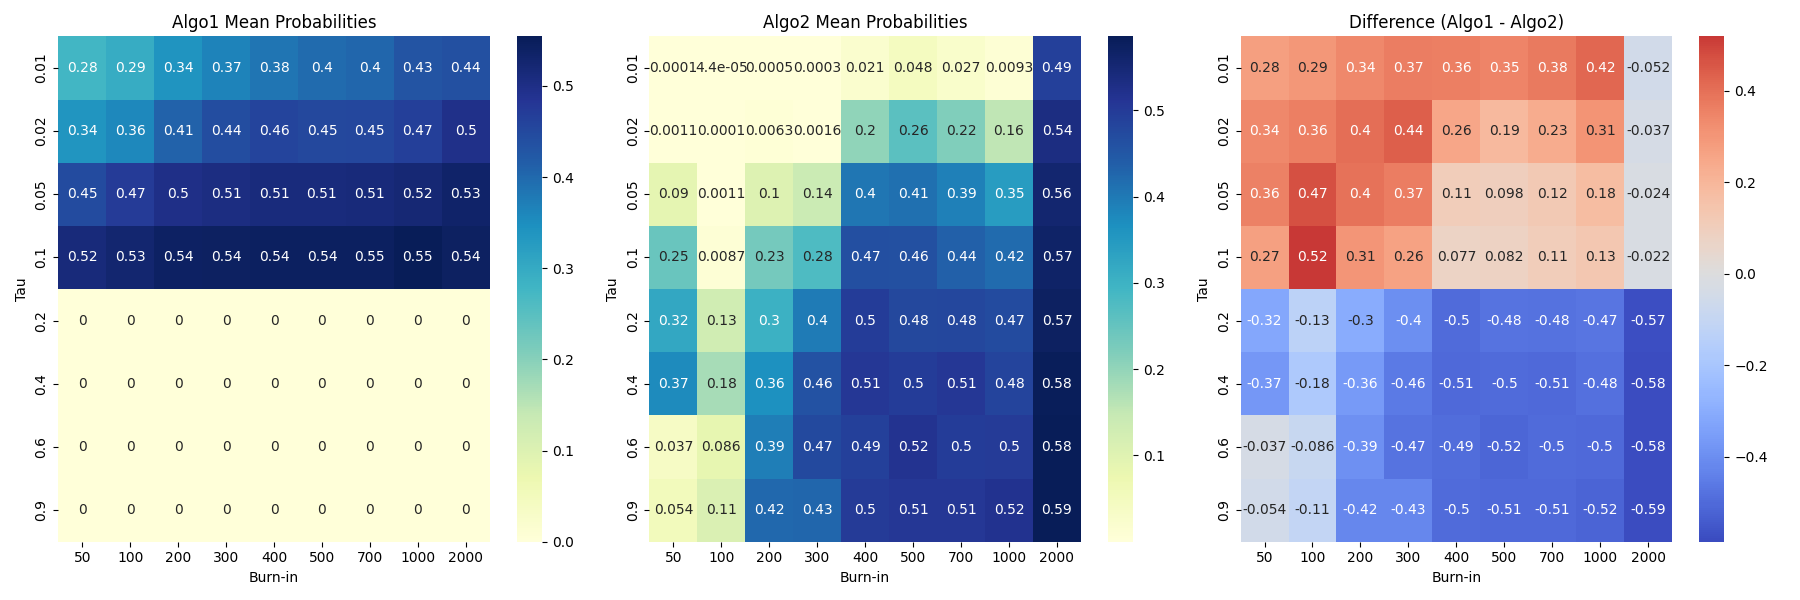
\includegraphics[width=\textwidth]{TASK-0-1/heatmap_prob.png}
  \caption{Heatmap showing the mean probability across various burn-in values and the number of samples for both the algorithms}
\end{figure}

Firstly, we observe that maxima of this probability is detected around $\tau = 0.1$, for both the algorithms, across various burn-in values.


Also, the probabilities typically increase, as we have more burn-in samples (which is actually obvious, because the actual samples are generated after this burn-in period, so less likely samples are already rejected).


Next, we used t-Sne, to plot these high dimensional samples into 1-D or 2-D. Here we show some of the results. Each image has samples plotted from both the algorithms:

\begin{figure}[H]
  \centering
  \begin{minipage}{0.38\textwidth}
    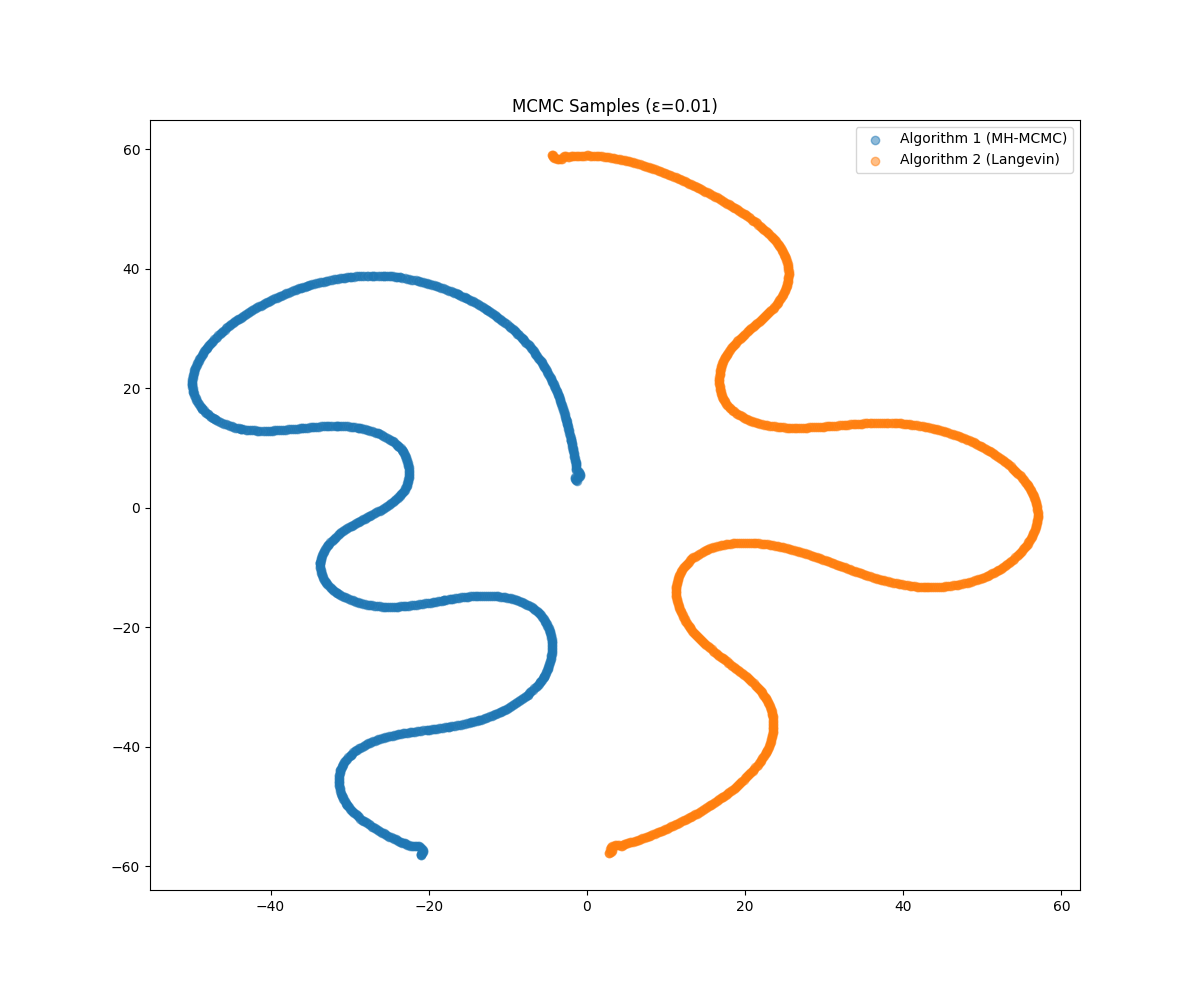
\includegraphics[width=\linewidth]{TASK-0-1/images/samples_eps0.01_n1000_burn1000_tsne_2d.png}
    % \caption*{(a) }
  \end{minipage}
  \hfill
  \begin{minipage}{0.38\textwidth}
    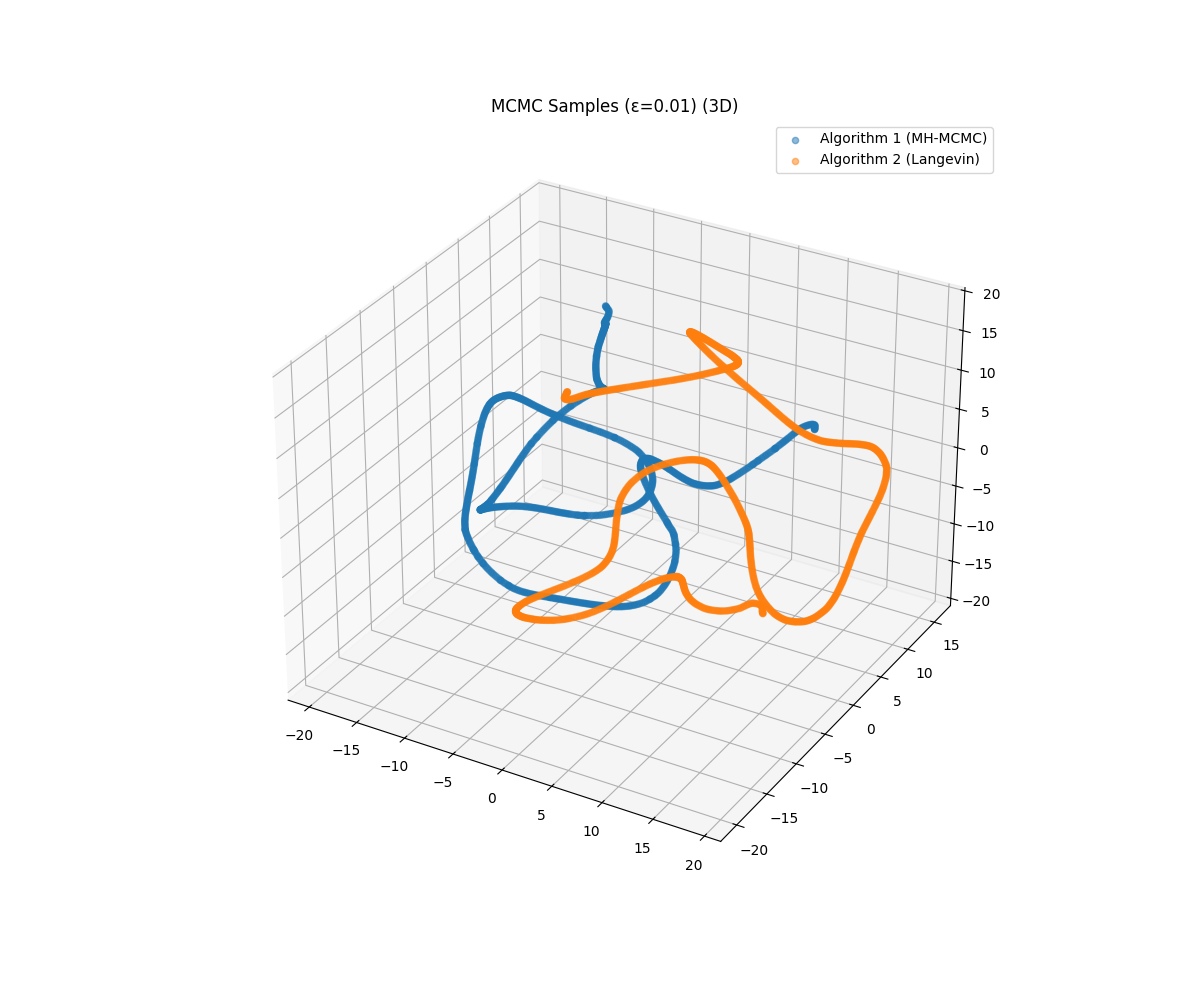
\includegraphics[width=\linewidth]{TASK-0-1/images/samples_eps0.01_n1000_burn1000_tsne_3d.png}
    % \caption*{(b) $\tau = 0.01$, Number of samples = 1000, Burn-in period = 1000}
  \end{minipage}
  \caption{$\tau = 0.01$, Number of samples = 1000, burn-in samples = 1000}
\end{figure}


\begin{figure}[H]
  \centering
  \begin{minipage}{0.38\textwidth}
    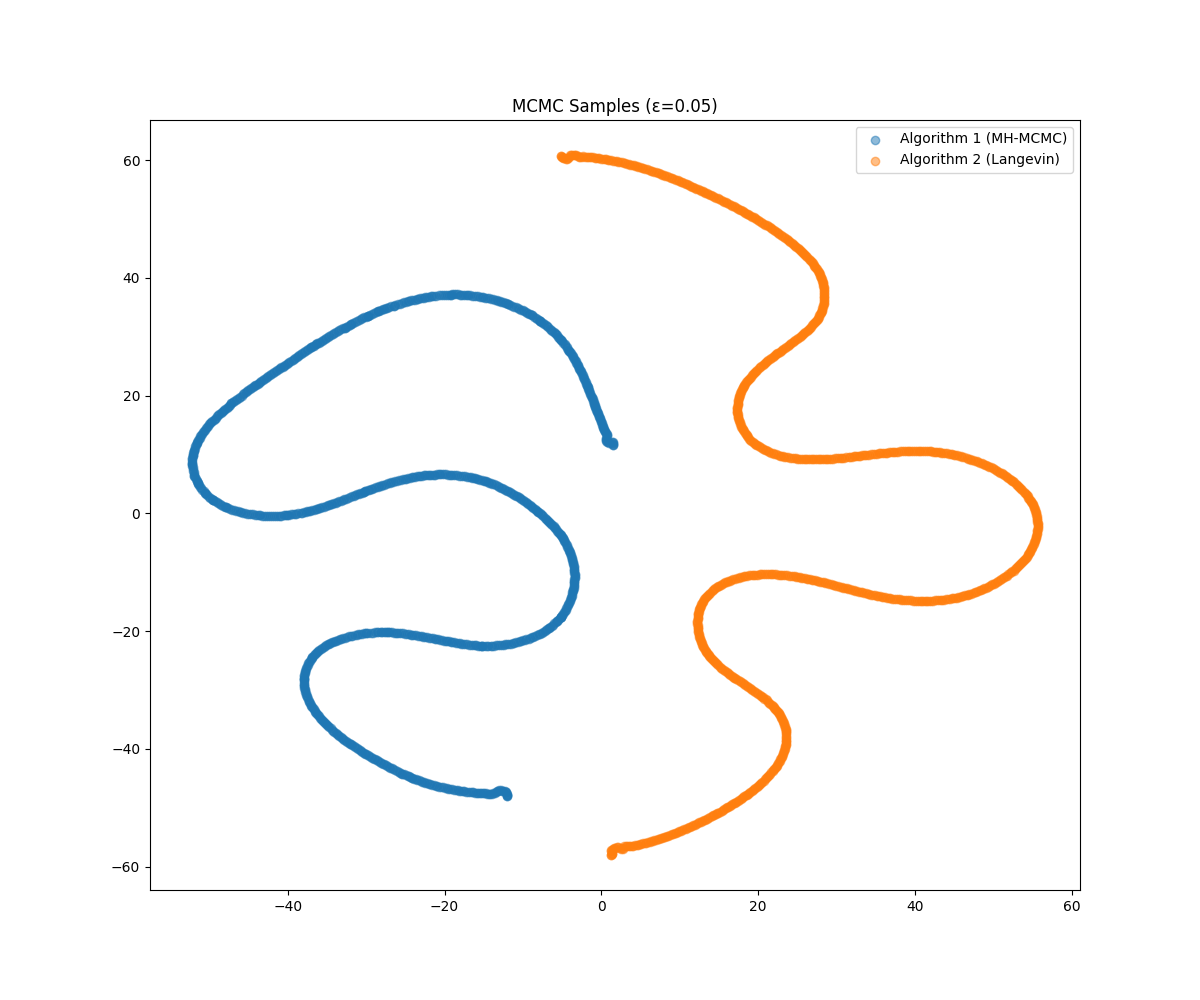
\includegraphics[width=\linewidth]{TASK-0-1/images/samples_eps0.05_n1000_burn1000_tsne_2d.png}
    % \caption*{(a) }
  \end{minipage}
  \hfill
  \begin{minipage}{0.38\textwidth}
    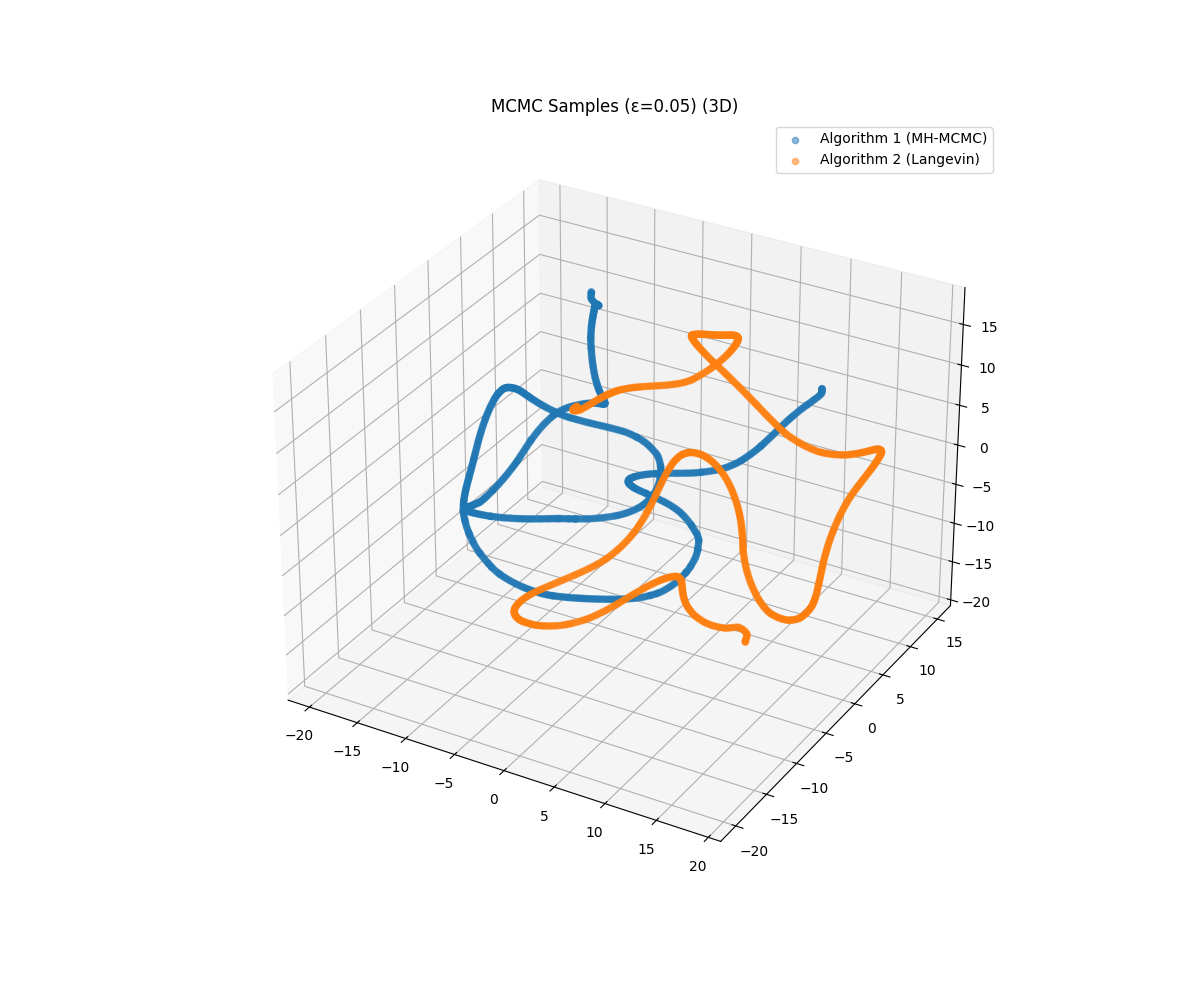
\includegraphics[width=\linewidth]{TASK-0-1/images/samples_eps0.05_n1000_burn1000_tsne_3d.png}
    % \caption*{(b) $\tau = 0.01$, Number of samples = 1000, Burn-in period = 1000}
  \end{minipage}
  \caption{$\tau = 0.05$, Number of samples = 1000, burn-in samples = 1000}
\end{figure}

\begin{figure}[H]
  \centering
  \begin{minipage}{0.38\textwidth}
    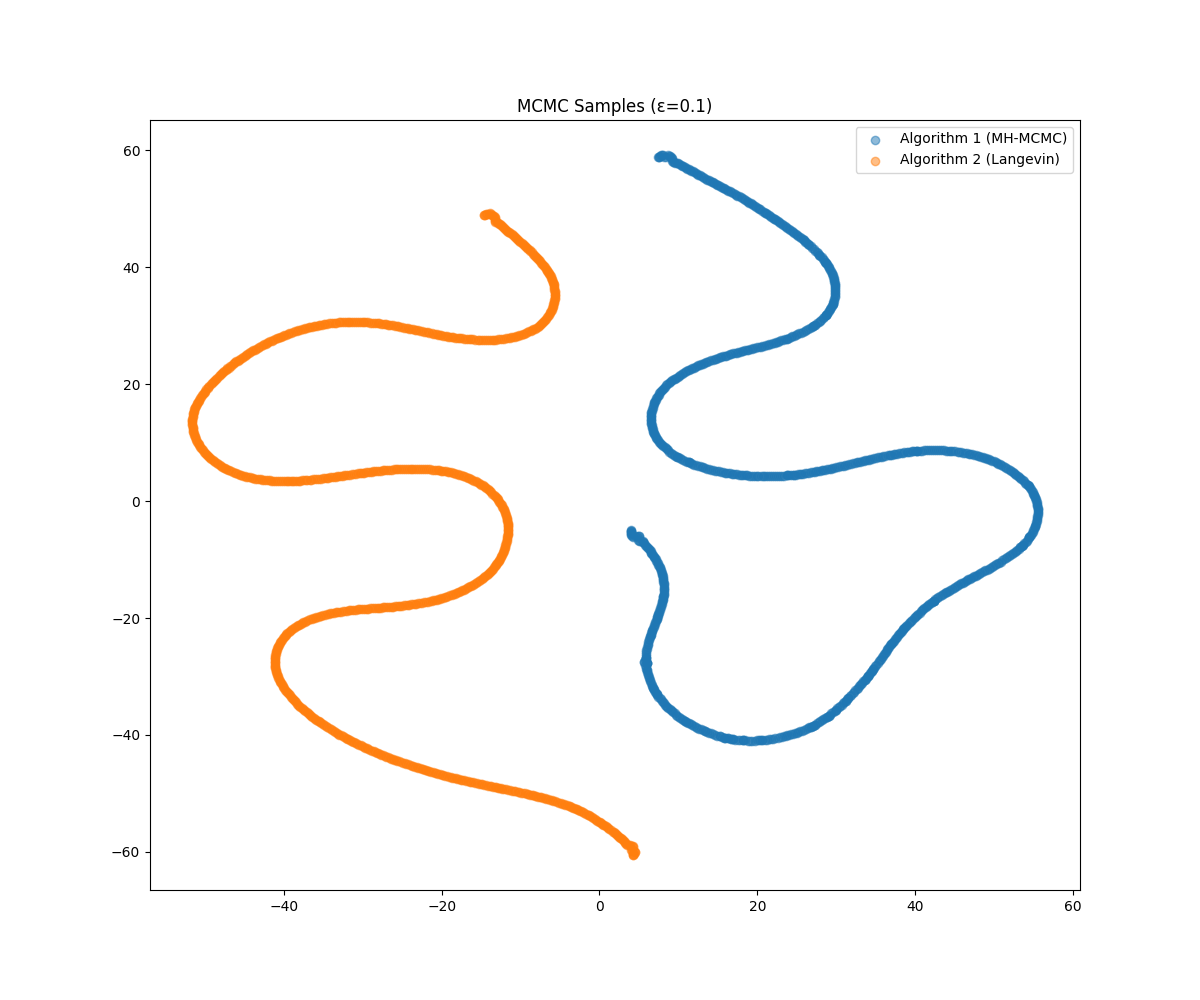
\includegraphics[width=\linewidth]{TASK-0-1/images/samples_eps0.1_n1000_burn50_tsne_2d.png}
  \end{minipage}
  \hfill
  \begin{minipage}{0.38\textwidth}
    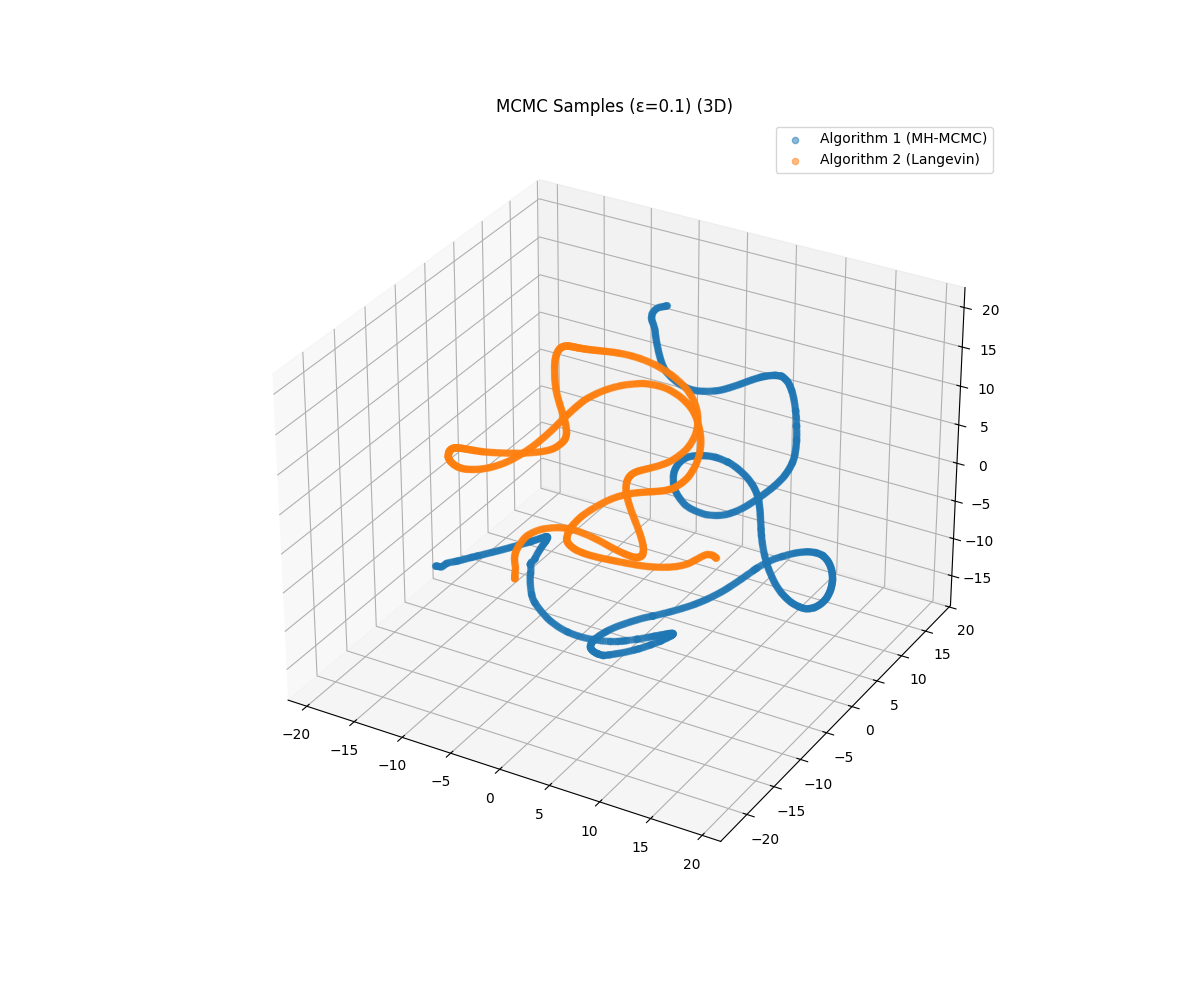
\includegraphics[width=\linewidth]{TASK-0-1/images/samples_eps0.1_n1000_burn50_tsne_3d.png}
  \end{minipage}
  \caption{$\tau = 0.1$, Number of samples = 1000, burn-in samples = 50}
\end{figure}


\begin{figure}[H]
  \centering
  \begin{minipage}{0.38\textwidth}
    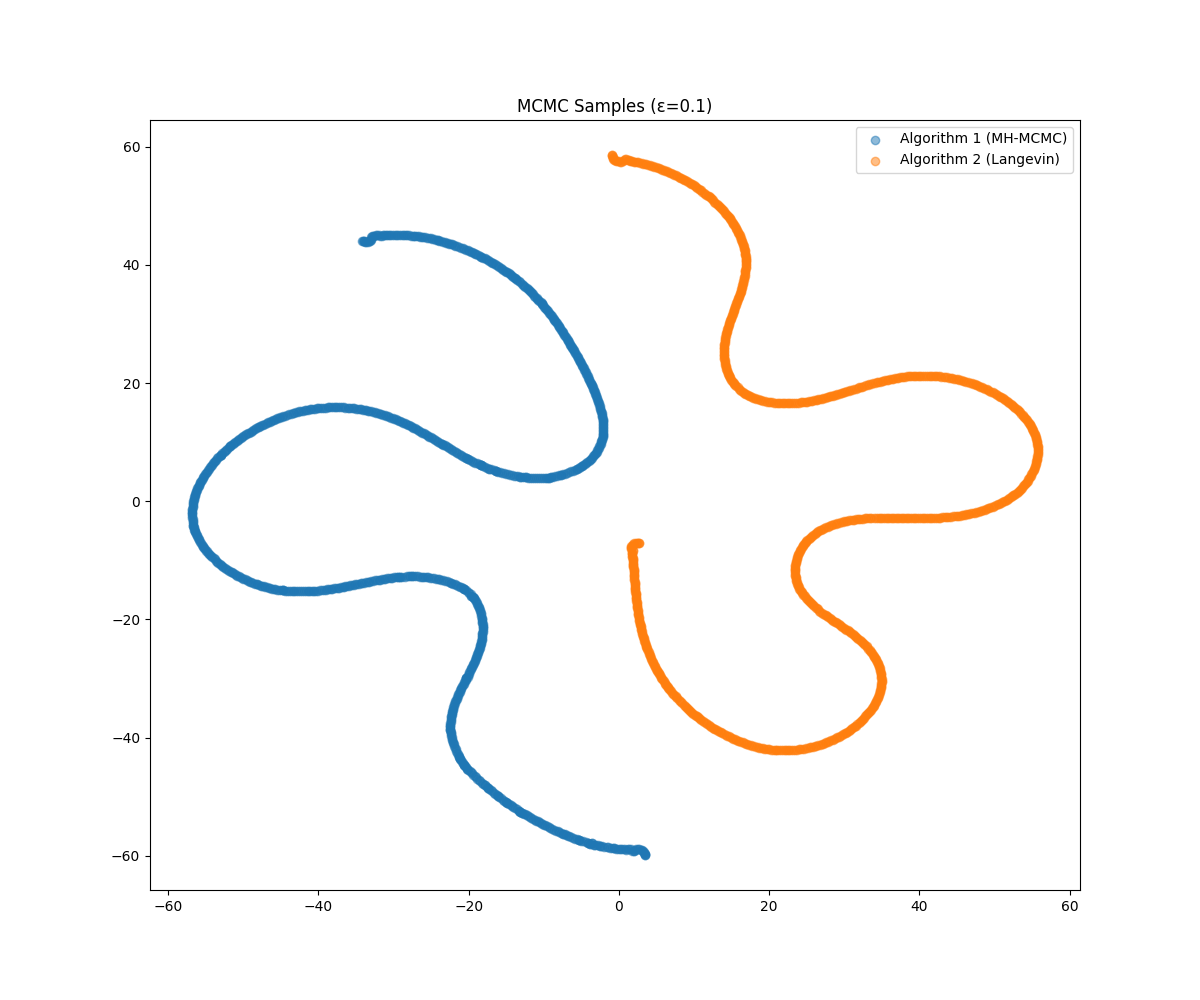
\includegraphics[width=\linewidth]{TASK-0-1/images/samples_eps0.1_n1000_burn200_tsne_2d.png}
  \end{minipage}
  \hfill
  \begin{minipage}{0.38\textwidth}
    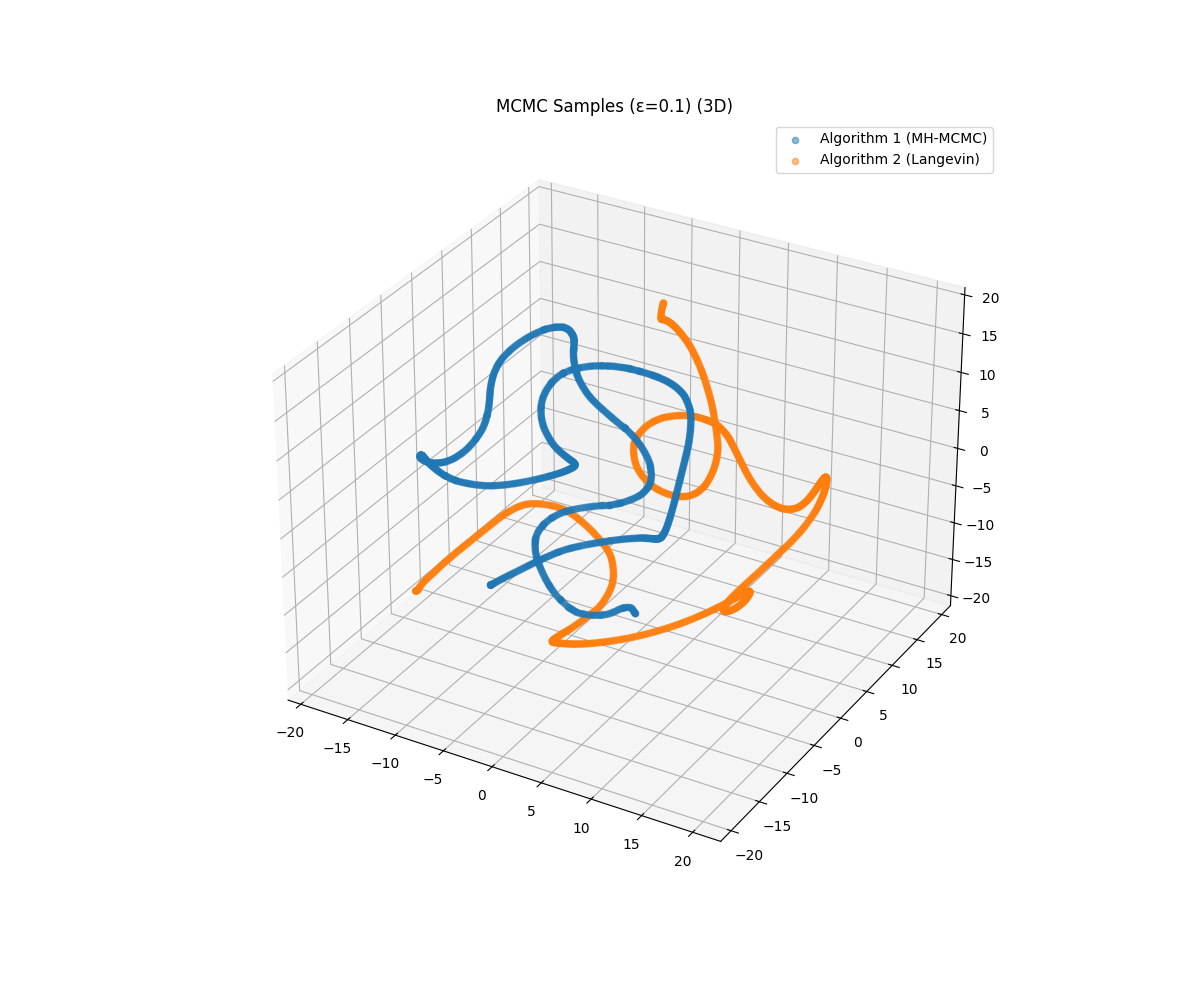
\includegraphics[width=\linewidth]{TASK-0-1/images/samples_eps0.1_n1000_burn200_tsne_3d.png}
  \end{minipage}
  \caption{$\tau = 0.1$, Number of samples = 1000, burn-in samples = 200}
\end{figure}

\begin{figure}[H]
  \centering
  \begin{minipage}{0.38\textwidth}
    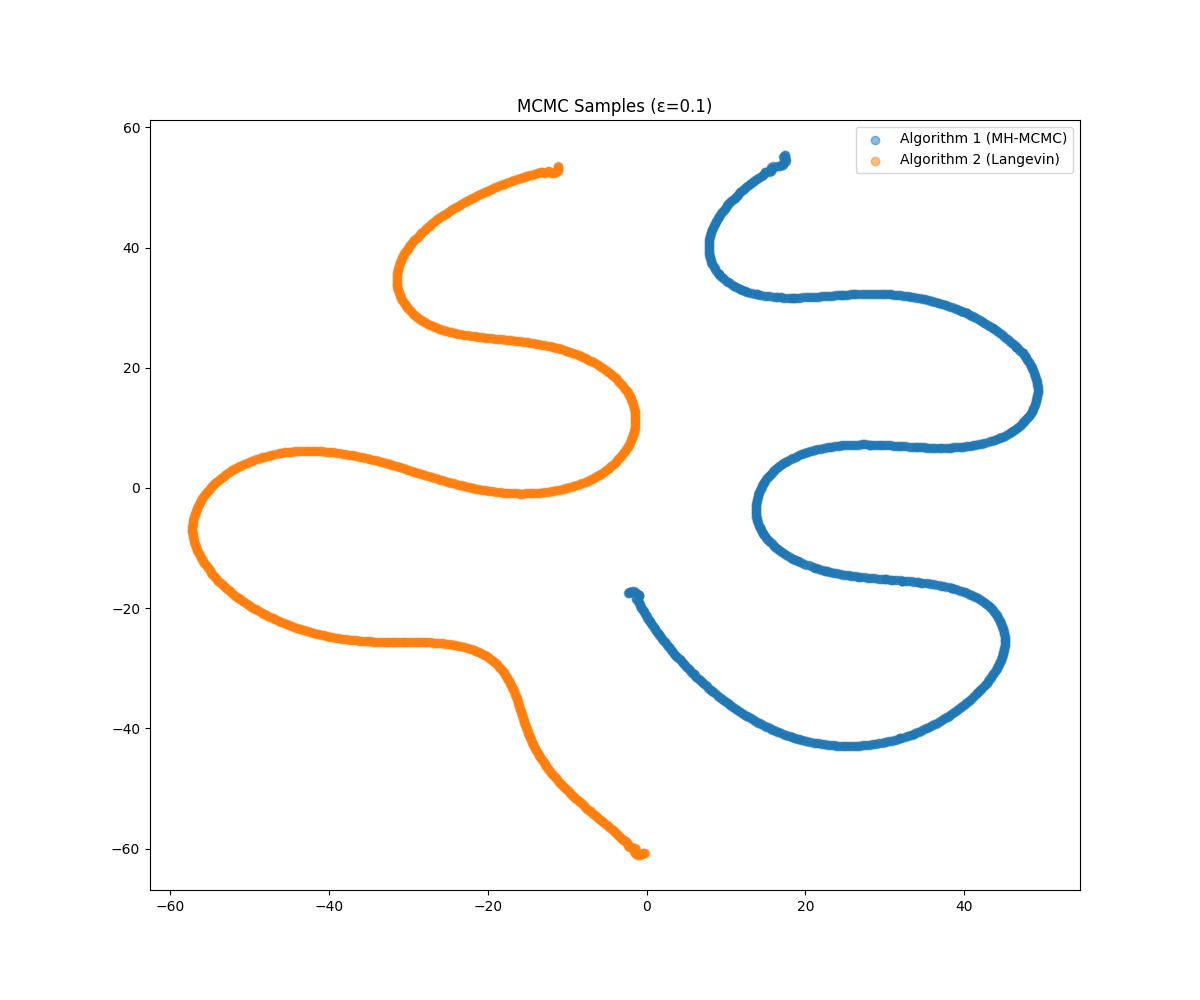
\includegraphics[width=\linewidth]{TASK-0-1/images/samples_eps0.1_n1000_burn500_tsne_2d.png}
  \end{minipage}
  \hfill
  \begin{minipage}{0.38\textwidth}
    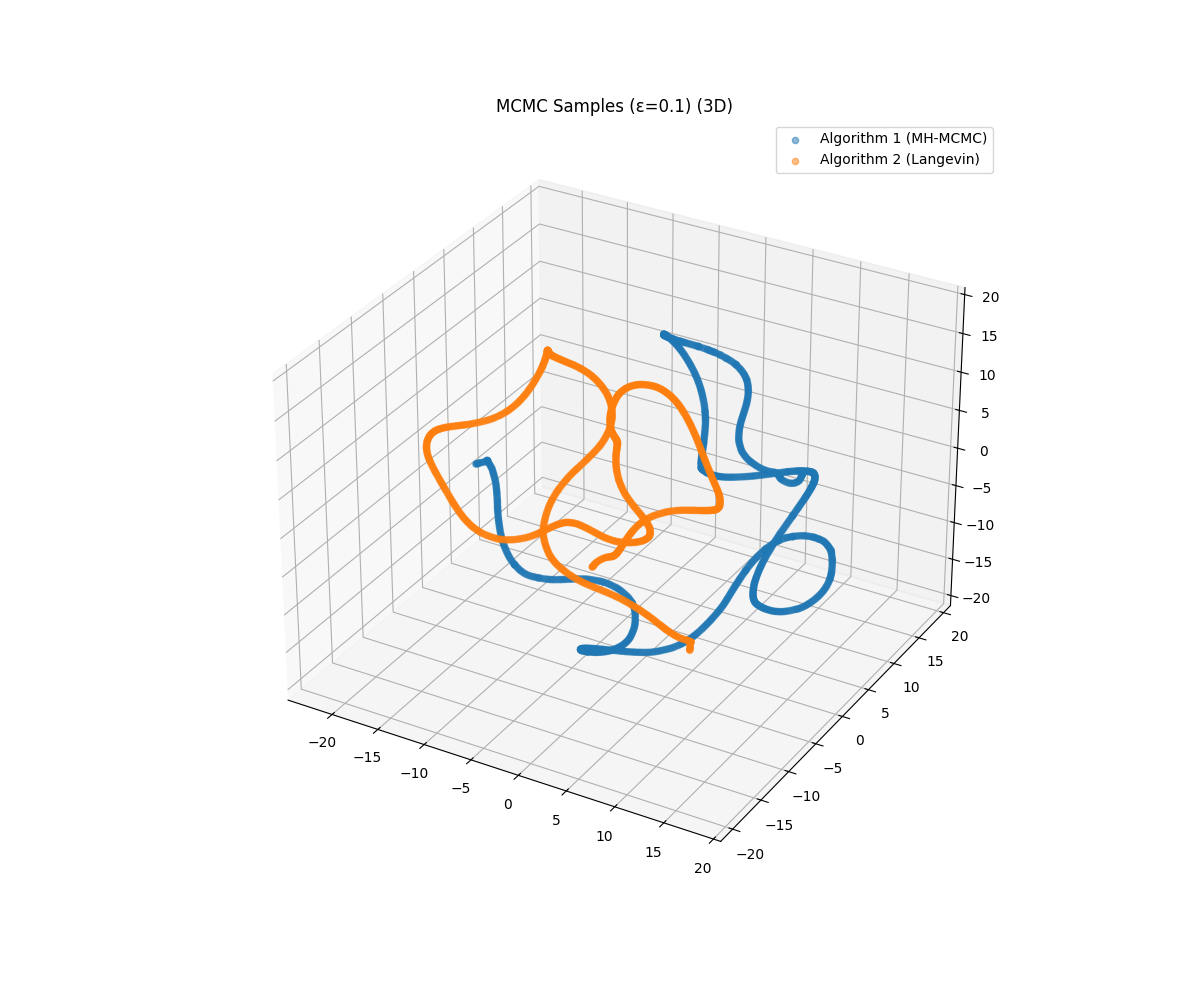
\includegraphics[width=\linewidth]{TASK-0-1/images/samples_eps0.1_n1000_burn500_tsne_3d.png}
  \end{minipage}
  \caption{$\tau = 0.1$, Number of samples = 1000, burn-in samples = 500}
\end{figure}


\begin{figure}[H]
  \centering
  \begin{minipage}{0.38\textwidth}
    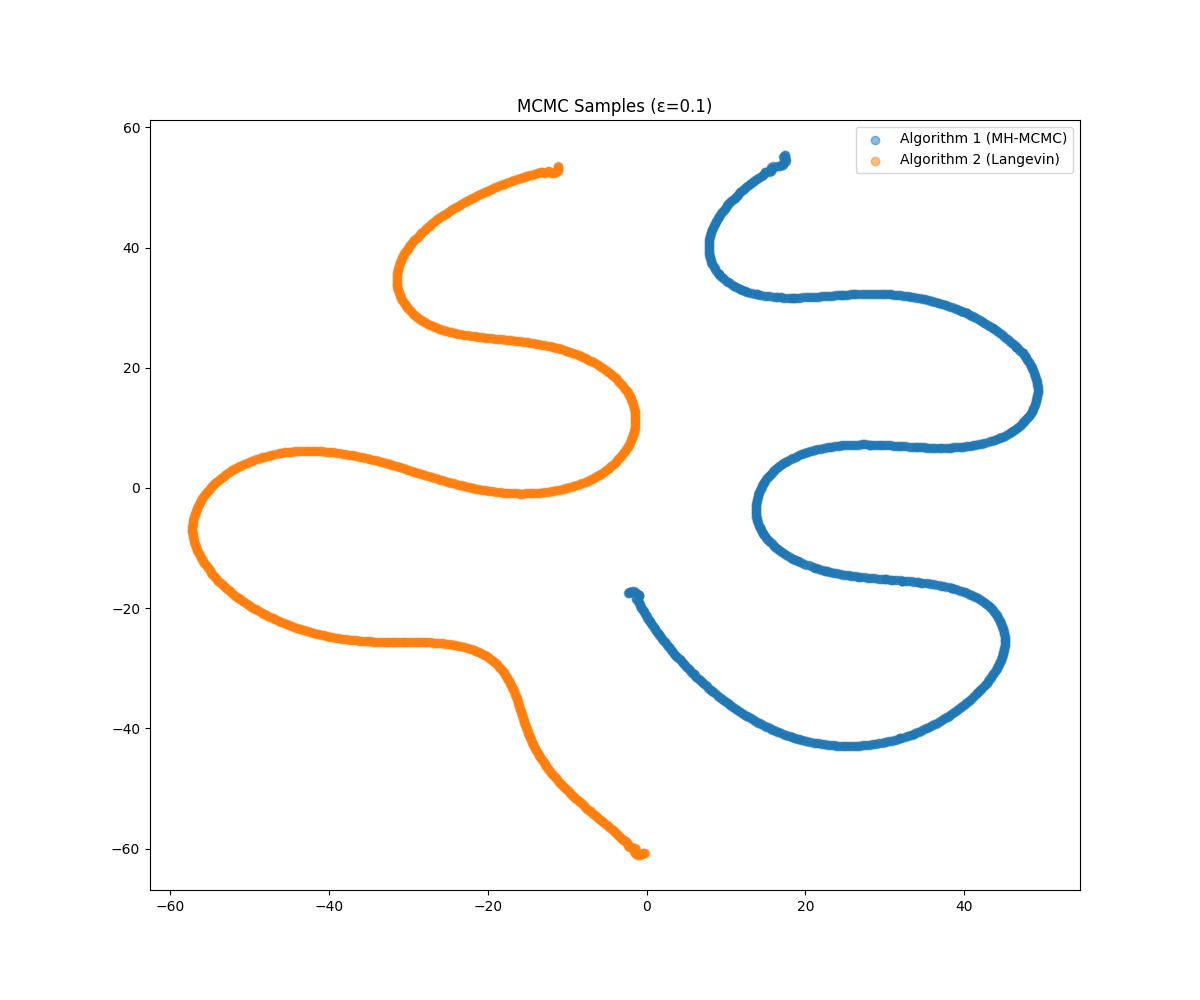
\includegraphics[width=\linewidth]{TASK-0-1/images/samples_eps0.1_n1000_burn500_tsne_2d.png}
  \end{minipage}
  \hfill
  \begin{minipage}{0.38\textwidth}
    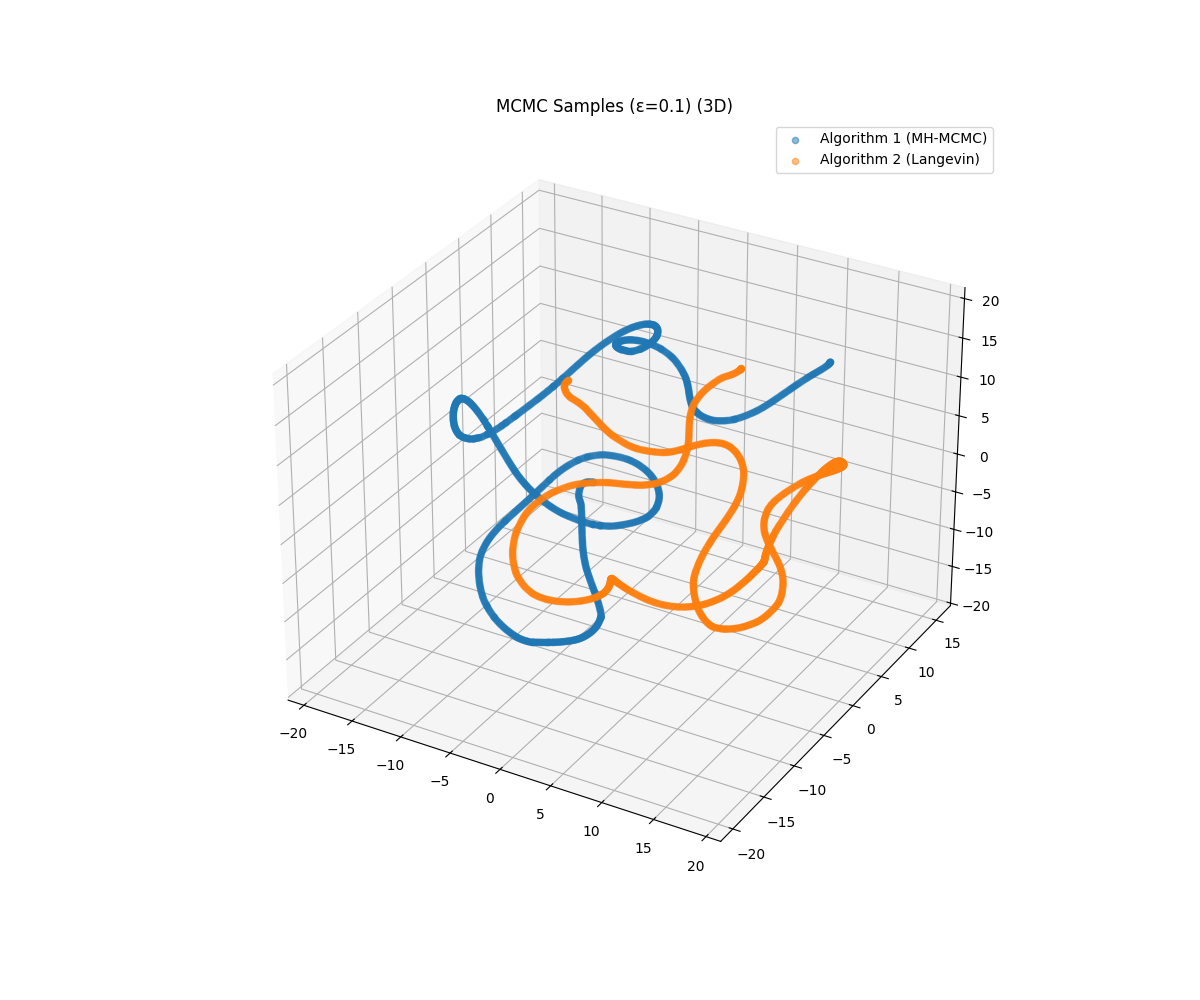
\includegraphics[width=\linewidth]{TASK-0-1/images/samples_eps0.1_n1000_burn1000_tsne_3d.png}
  \end{minipage}
  \caption{$\tau = 0.1$, Number of samples = 1000, burn-in samples = 1000}
\end{figure}


\begin{figure}[H]
  \centering
  \begin{minipage}{0.38\textwidth}
    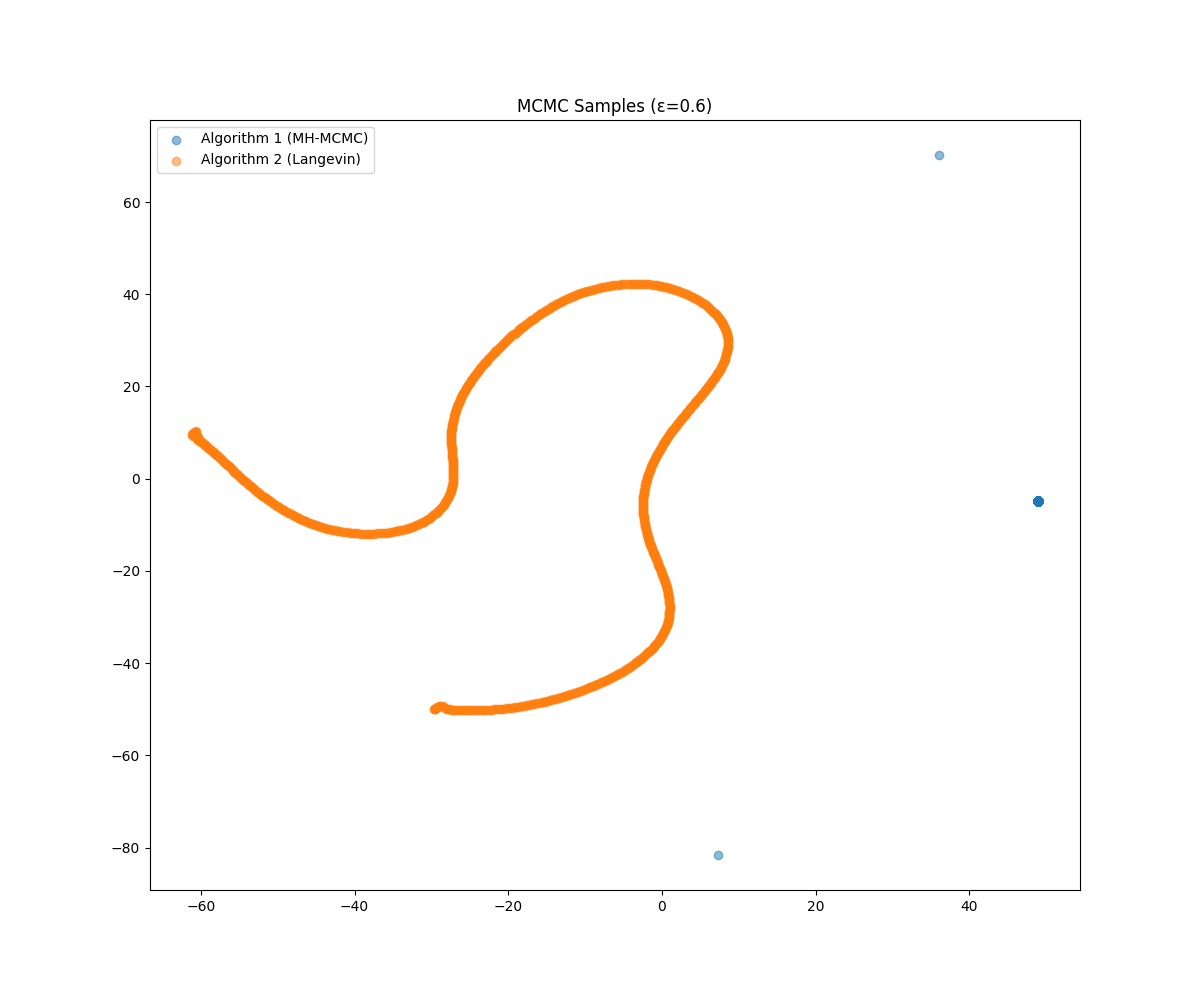
\includegraphics[width=\linewidth]{TASK-0-1/images/samples_eps0.6_n1000_burn500_tsne_2d.png}
  \end{minipage}
  \hfill
  \begin{minipage}{0.38\textwidth}
    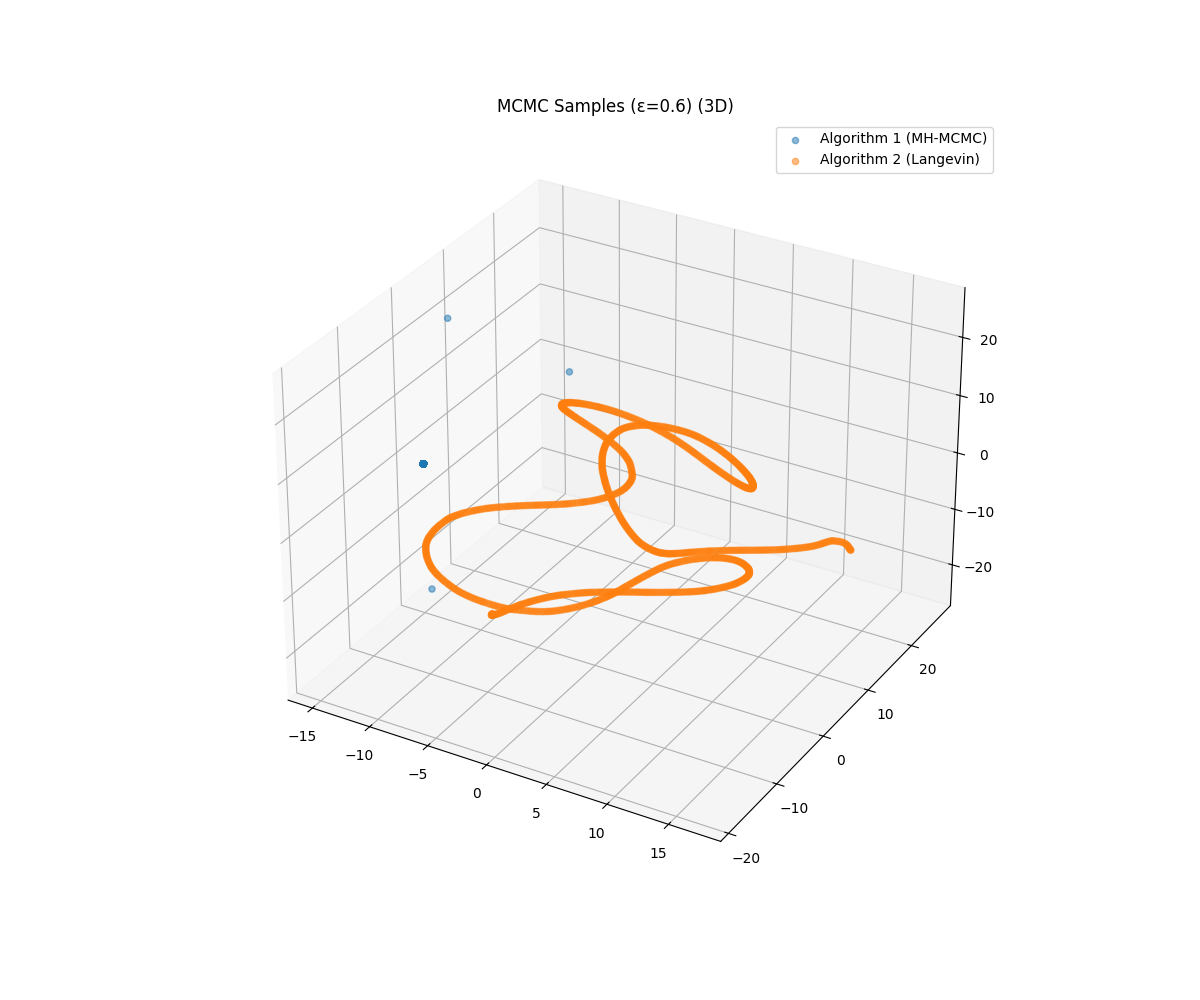
\includegraphics[width=\linewidth]{TASK-0-1/images/samples_eps0.6_n1000_burn1000_tsne_3d.png}
  \end{minipage}
  \caption{$\tau = 0.6$, Number of samples = 1000, burn-in samples = 1000}
\end{figure}



As, we can see, algorithm-1 performs quite badly, in case the value of $\tau$ is more than $0.3$ (the acceptance probability is roughly 0, so we aren't able to move much from our initial guess). The detailed result are present in the file \texttt{TASK-0-1/out}, which shows the burn-in times, along with acceptance probabilities, for all the experiments done.

\section*{Task 2: Approximating a Black-Box Function Using Gaussian Processes}

The following plots show the predicted mean and standard deviation of the Gaussian Process (GP) model using different combinations of:
\begin{itemize}
    \item \textbf{Kernels:} RBF, Matérn, Rational Quadratic
    \item \textbf{Sample Sizes:} 10, 20, 50, 100
    \item \textbf{Acquisition Functions:} Expected Improvement (EI), Probability of Improvement (PI), Random
\end{itemize}

Each row contains the true Branin-Hoo function, the predicted mean and corresponding uncertainty (standard deviation) for one configuration. All image files are stored in \texttt{Task-02/images}.

% ========== RBF Kernel ==========
\subsection*{Kernel: Matérn}

\subsubsection*{Acquisition: Expected Improvement (EI)}
\begin{figure}[H]
\centering
\begin{subfigure}{0.3\textwidth}
  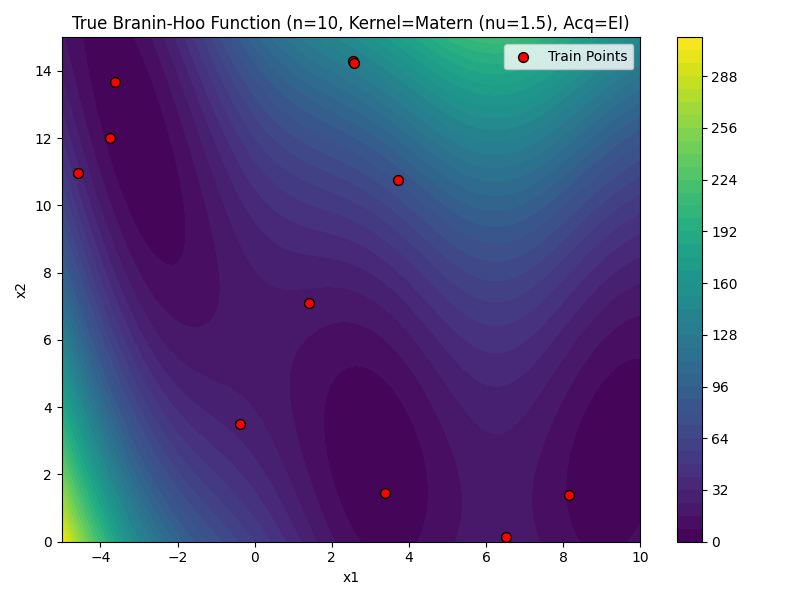
\includegraphics[width=\linewidth]{Task-02/images/true_function_matern_n10_EI.png}
  \caption{True Branin-Hoo, $n=10$}
\end{subfigure}
\begin{subfigure}{0.3\textwidth}
    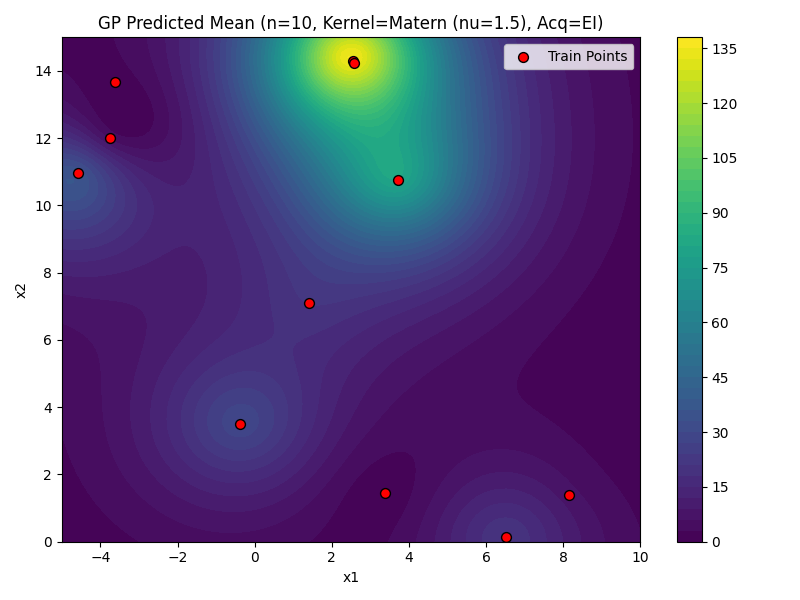
\includegraphics[width=\linewidth]{Task-02/images/gp_mean_matern_n10_EI.png}
    \caption{Mean, $n=10$}
\end{subfigure}
\begin{subfigure}{0.3\textwidth}
    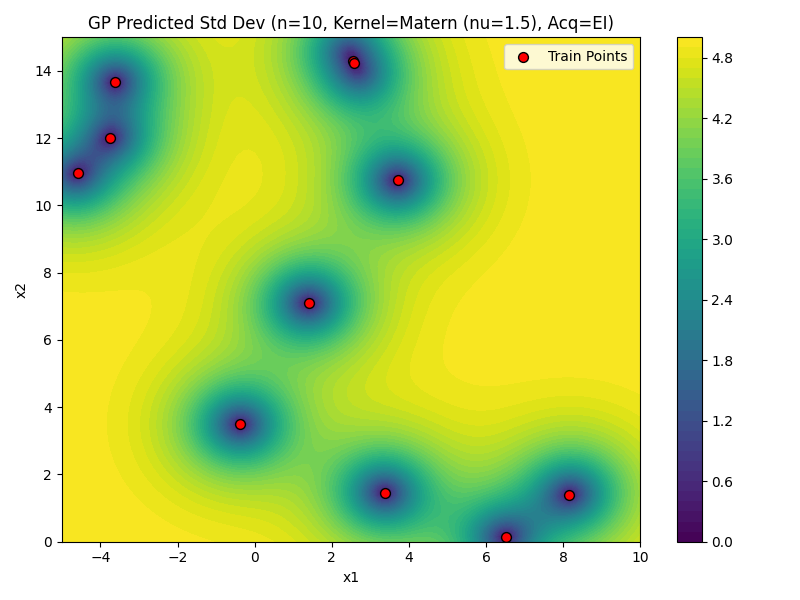
\includegraphics[width=\linewidth]{Task-02/images/gp_std_matern_n10_EI.png}
    \caption{Std, $n=10$}
\end{subfigure}

\begin{subfigure}{0.3\textwidth}
  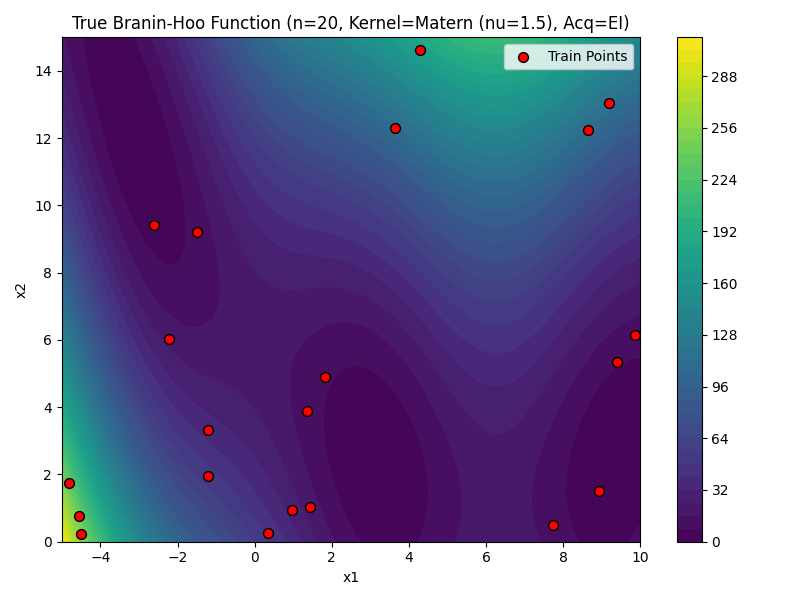
\includegraphics[width=\linewidth]{Task-02/images/true_function_matern_n20_EI.png}
  \caption{True Branin-Hoo, $n=20$}
\end{subfigure}
\begin{subfigure}{0.3\textwidth}
    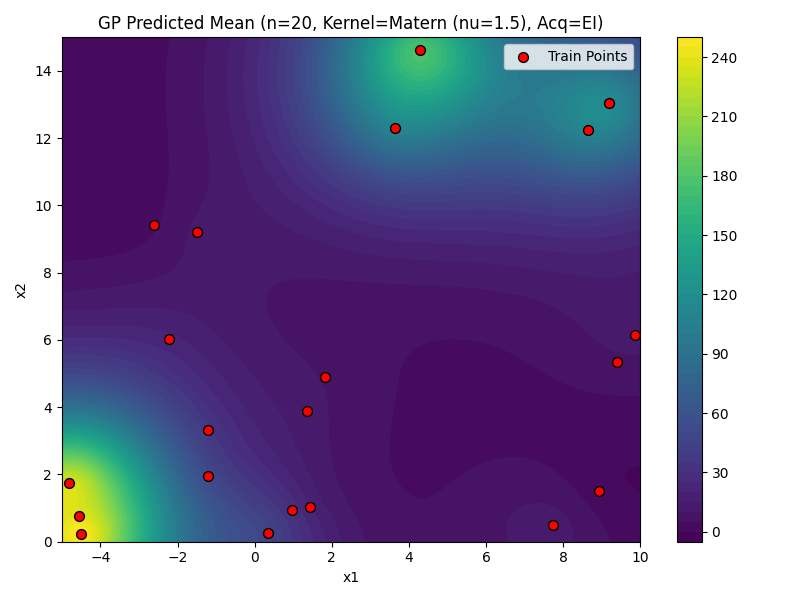
\includegraphics[width=\linewidth]{Task-02/images/gp_mean_matern_n20_EI.png}
    \caption{Mean, $n=20$}
\end{subfigure}
\begin{subfigure}{0.3\textwidth}
    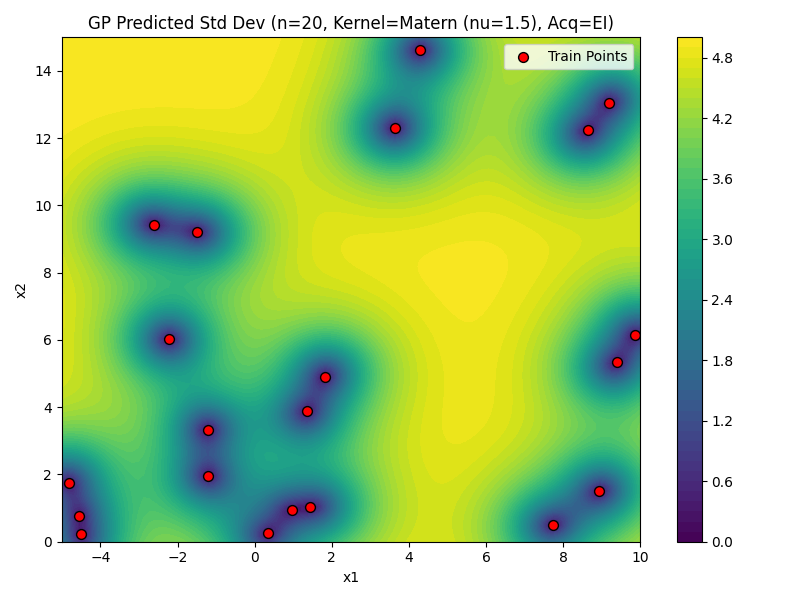
\includegraphics[width=\linewidth]{Task-02/images/gp_std_matern_n20_EI.png}
    \caption{Std, $n=20$}
\end{subfigure}

\begin{subfigure}{0.3\textwidth}
  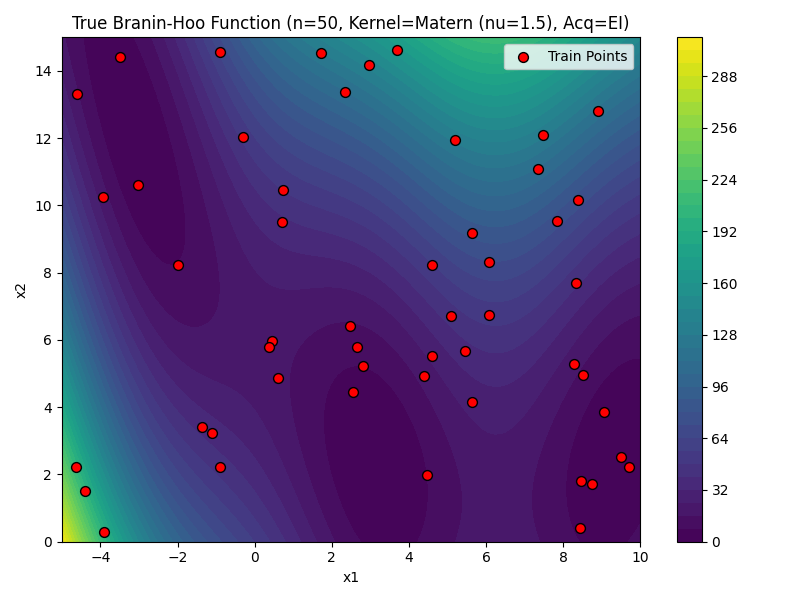
\includegraphics[width=\linewidth]{Task-02/images/true_function_matern_n50_EI.png}
  \caption{True Branin-Hoo, $n=50$}
\end{subfigure}
\begin{subfigure}{0.3\textwidth}
    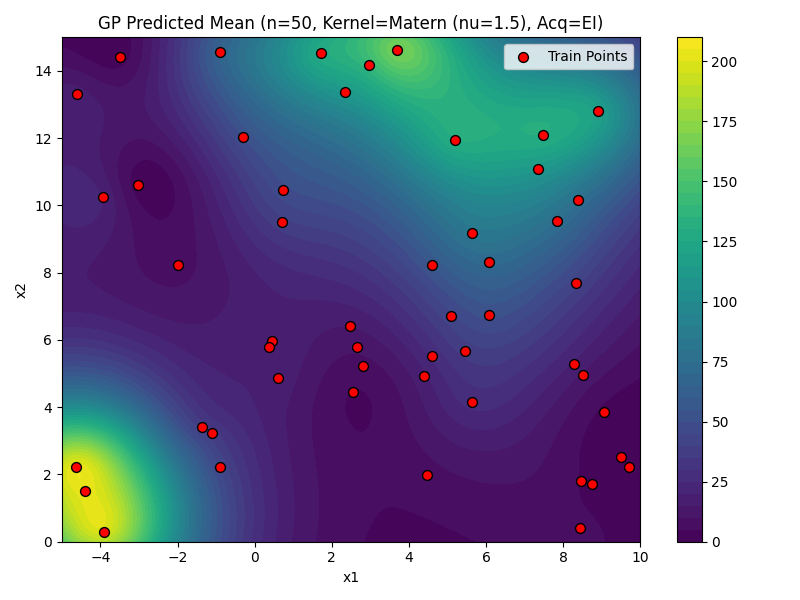
\includegraphics[width=\linewidth]{Task-02/images/gp_mean_matern_n50_EI.png}
    \caption{Mean, $n=50$}
\end{subfigure}
\begin{subfigure}{0.3\textwidth}
    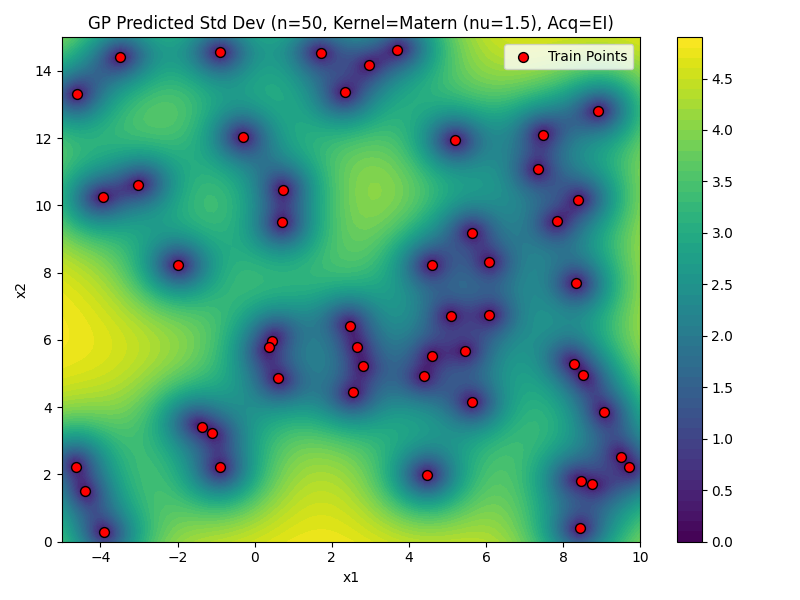
\includegraphics[width=\linewidth]{Task-02/images/gp_std_matern_n50_EI.png}
    \caption{Std, $n=50$}
\end{subfigure}

\begin{subfigure}{0.3\textwidth}
  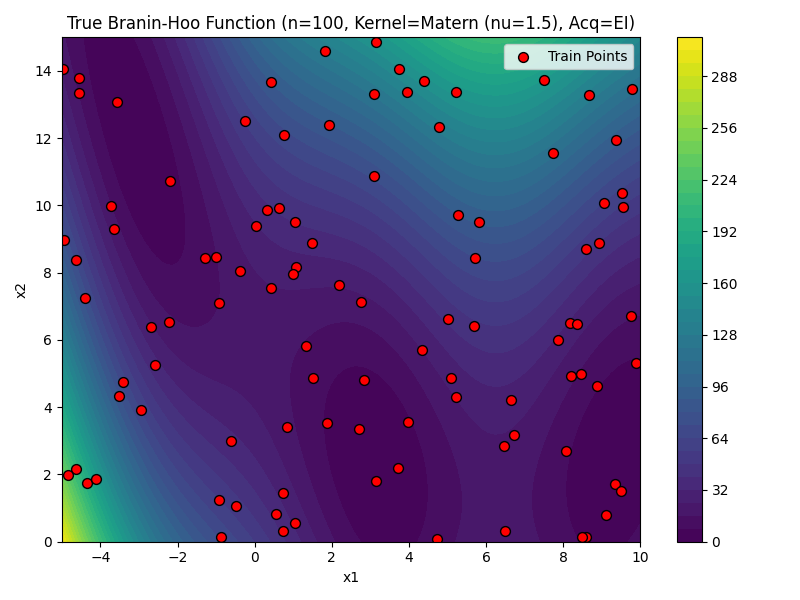
\includegraphics[width=\linewidth]{Task-02/images/true_function_matern_n100_EI.png}
  \caption{True Branin-Hoo, $n=100$}
\end{subfigure}
\begin{subfigure}{0.3\textwidth}
    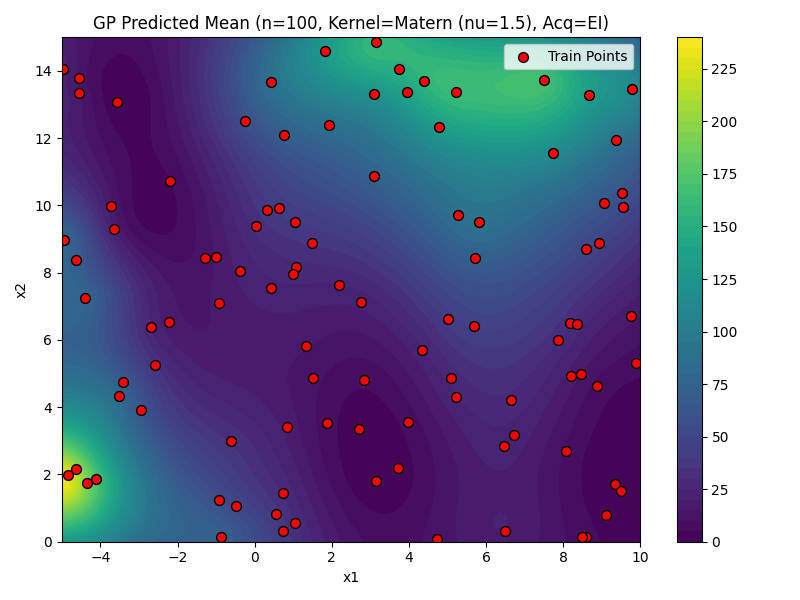
\includegraphics[width=\linewidth]{Task-02/images/gp_mean_matern_n100_EI.png}
    \caption{Mean, $n=100$}
\end{subfigure}
\begin{subfigure}{0.3\textwidth}
    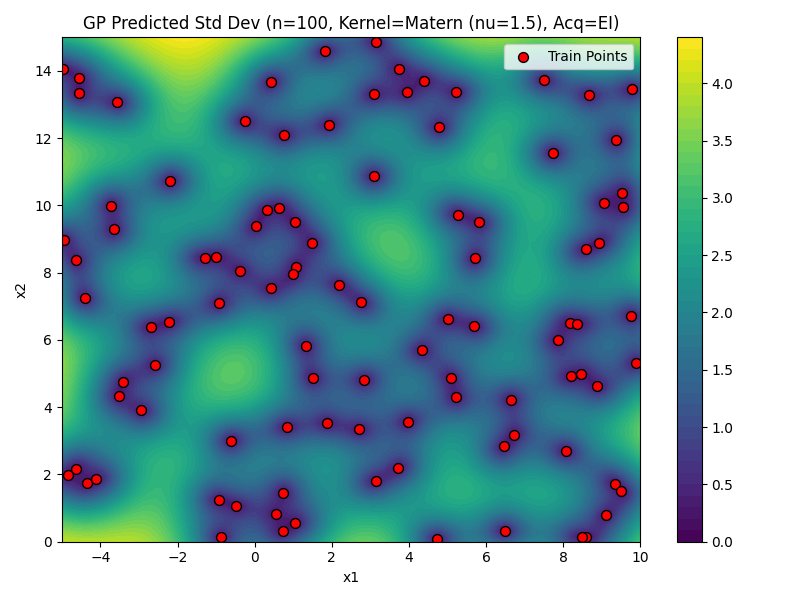
\includegraphics[width=\linewidth]{Task-02/images/gp_std_matern_n100_EI.png}
    \caption{Std, $n=100$}
\end{subfigure}
\end{figure}

\subsection*{Kernel: RBF}

\subsubsection*{Acquisition: Expected Improvement (EI)}
\begin{figure}[H]
\centering
\begin{subfigure}{0.3\textwidth}
  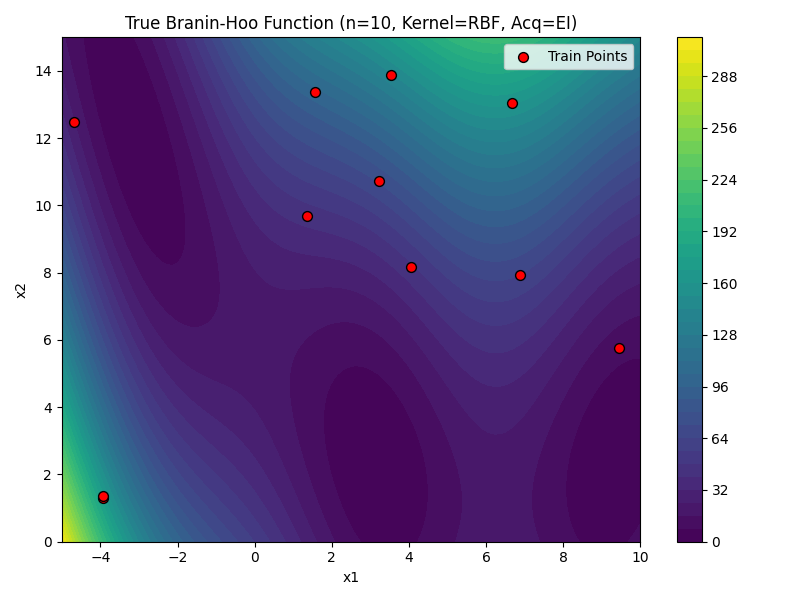
\includegraphics[width=\linewidth]{Task-02/images/true_function_rbf_n10_EI.png}
  \caption{True Branin-Hoo, $n=10$}
\end{subfigure}
\begin{subfigure}{0.3\textwidth}
    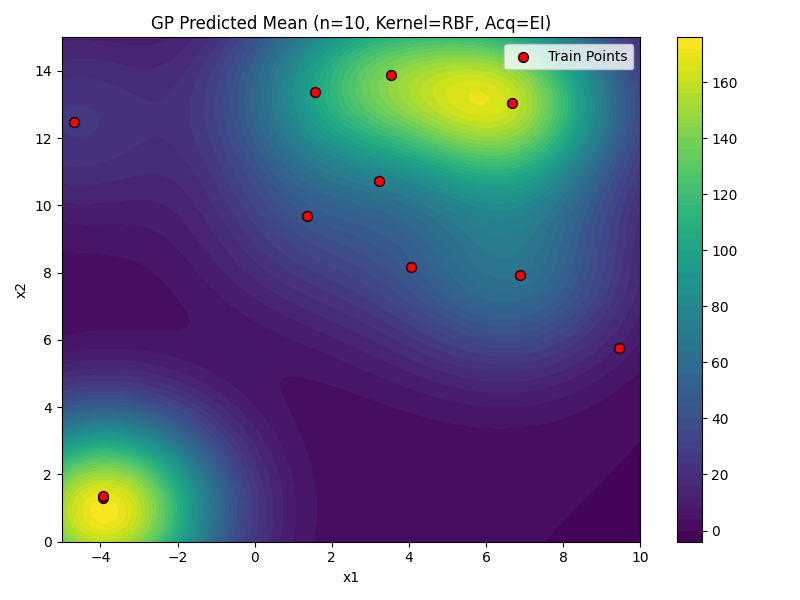
\includegraphics[width=\linewidth]{Task-02/images/gp_mean_rbf_n10_EI.png}
    \caption{Mean, $n=10$}
\end{subfigure}
\begin{subfigure}{0.3\textwidth}
    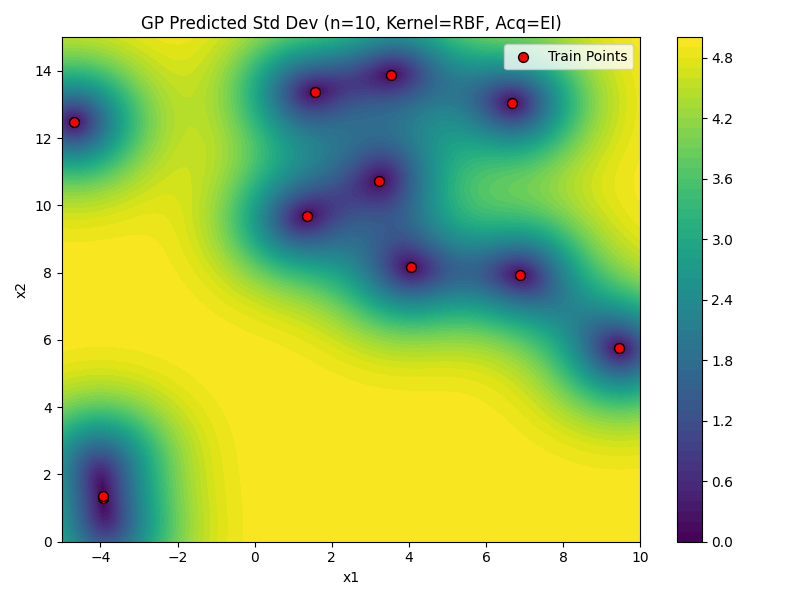
\includegraphics[width=\linewidth]{Task-02/images/gp_std_rbf_n10_EI.png}
    \caption{Std, $n=10$}
\end{subfigure}

\begin{subfigure}{0.3\textwidth}
  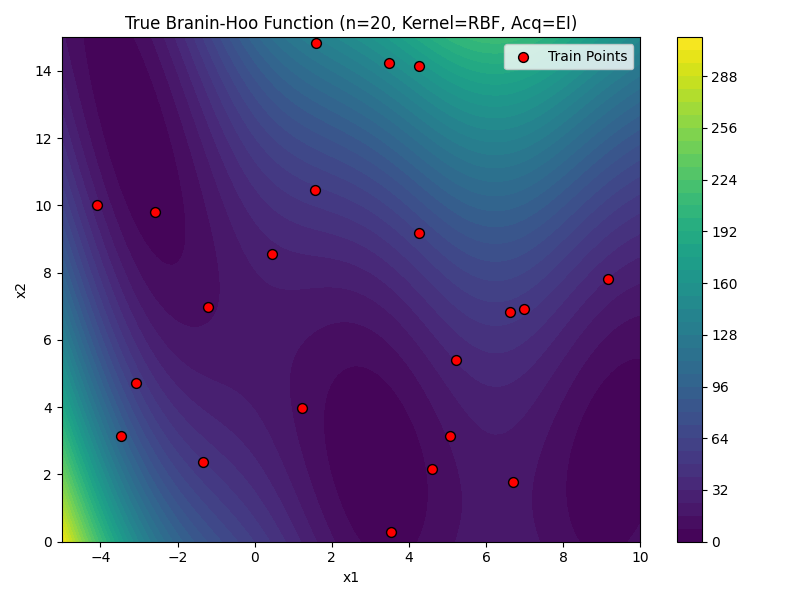
\includegraphics[width=\linewidth]{Task-02/images/true_function_rbf_n20_EI.png}
  \caption{True Branin-Hoo, $n=20$}
\end{subfigure}
\begin{subfigure}{0.3\textwidth}
    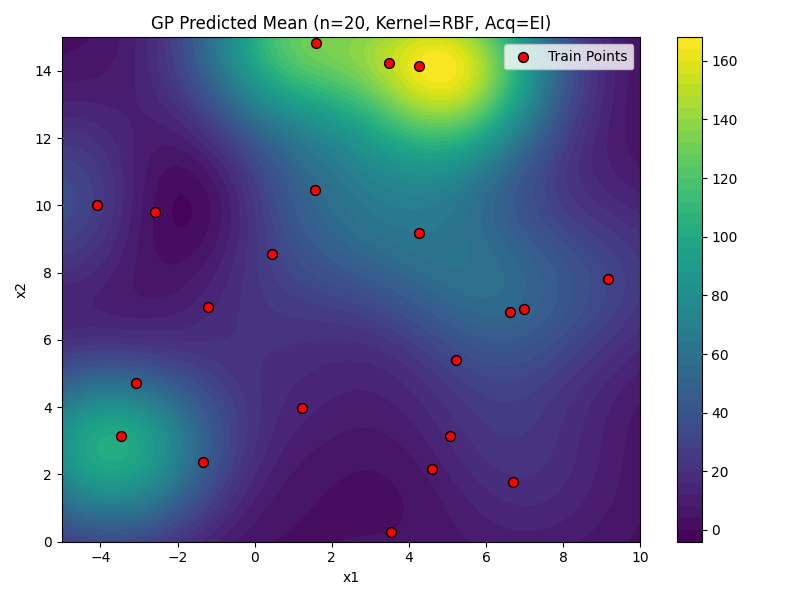
\includegraphics[width=\linewidth]{Task-02/images/gp_mean_rbf_n20_EI.png}
    \caption{Mean, $n=20$}
\end{subfigure}
\begin{subfigure}{0.3\textwidth}
    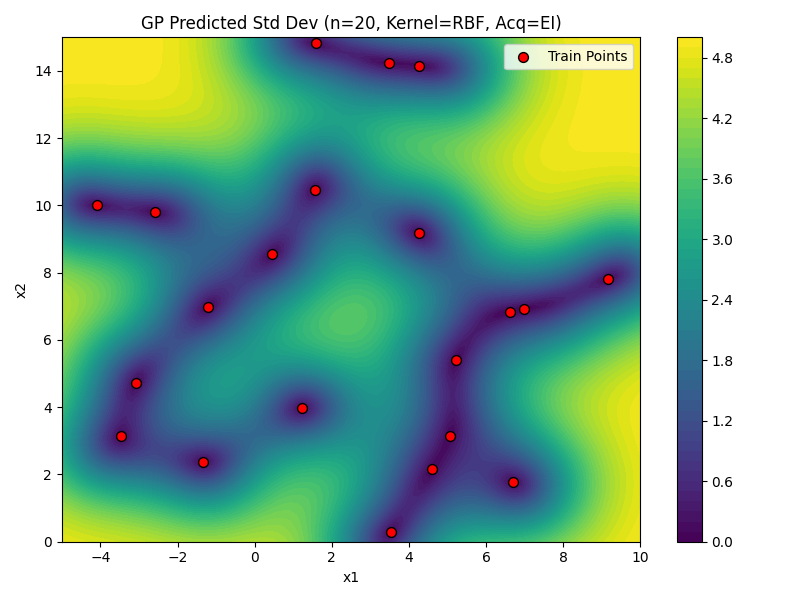
\includegraphics[width=\linewidth]{Task-02/images/gp_std_rbf_n20_EI.png}
    \caption{Std, $n=20$}
\end{subfigure}

\begin{subfigure}{0.3\textwidth}
  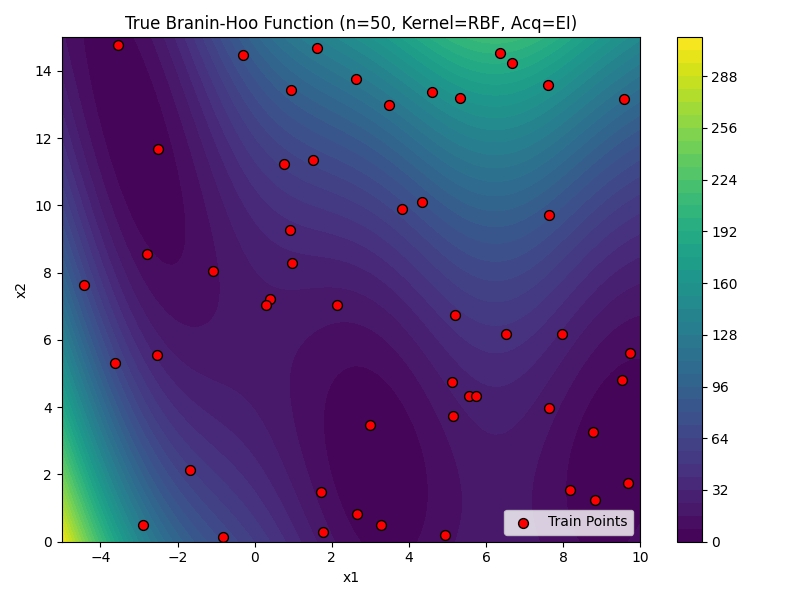
\includegraphics[width=\linewidth]{Task-02/images/true_function_rbf_n50_EI.png}
  \caption{True Branin-Hoo, $n=50$}
\end{subfigure}
\begin{subfigure}{0.3\textwidth}
    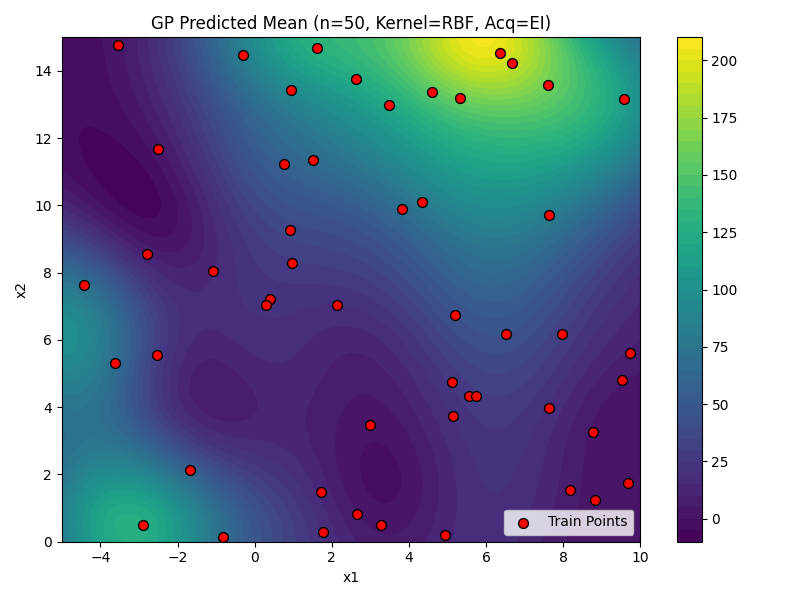
\includegraphics[width=\linewidth]{Task-02/images/gp_mean_rbf_n50_EI.png}
    \caption{Mean, $n=50$}
\end{subfigure}
\begin{subfigure}{0.3\textwidth}
    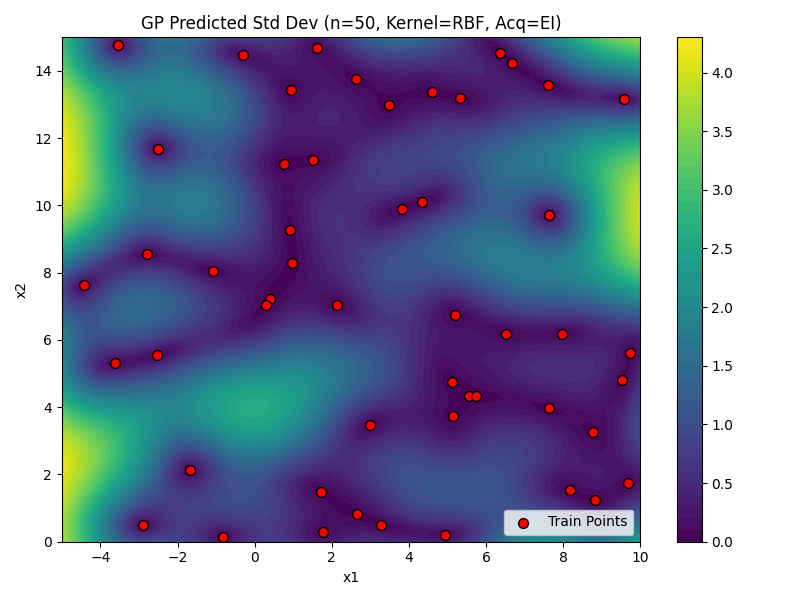
\includegraphics[width=\linewidth]{Task-02/images/gp_std_rbf_n50_EI.png}
    \caption{Std, $n=50$}
\end{subfigure}

\begin{subfigure}{0.3\textwidth}
  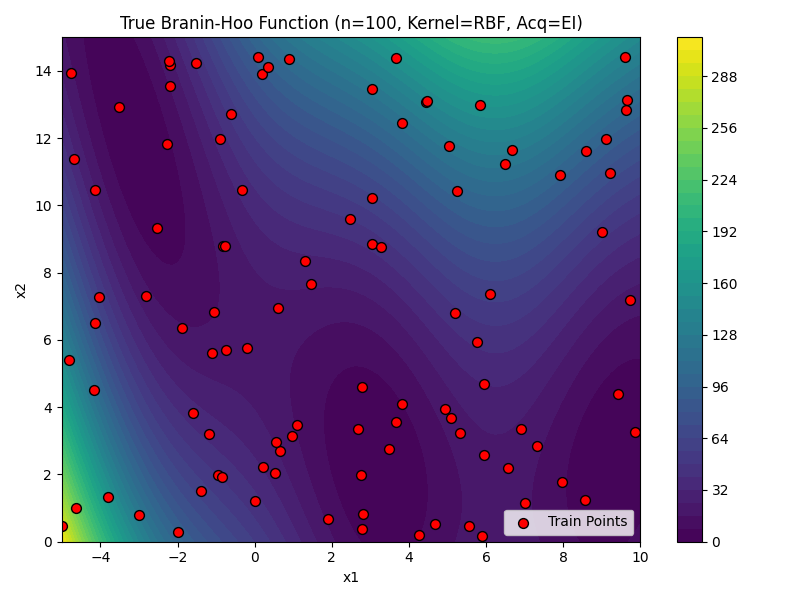
\includegraphics[width=\linewidth]{Task-02/images/true_function_rbf_n100_EI.png}
  \caption{True Branin-Hoo, $n=100$}
\end{subfigure}
\begin{subfigure}{0.3\textwidth}
    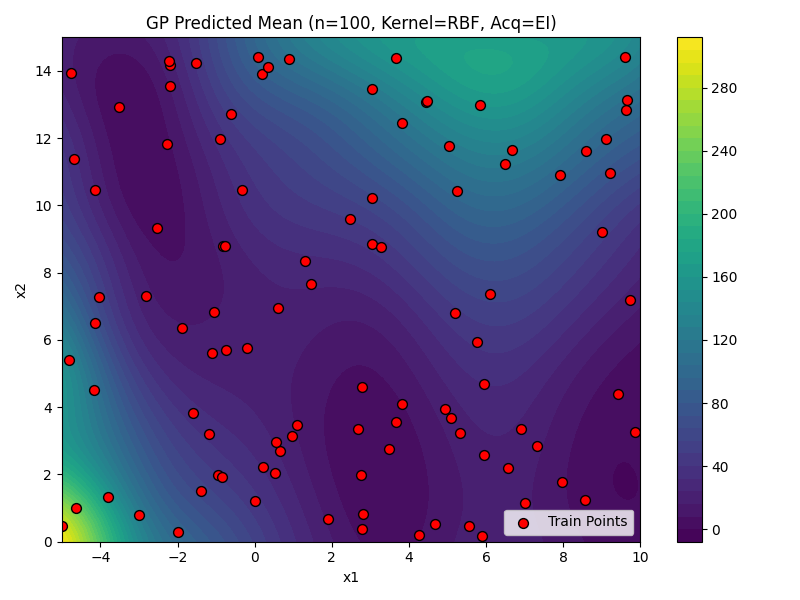
\includegraphics[width=\linewidth]{Task-02/images/gp_mean_rbf_n100_EI.png}
    \caption{Mean, $n=100$}
\end{subfigure}
\begin{subfigure}{0.3\textwidth}
    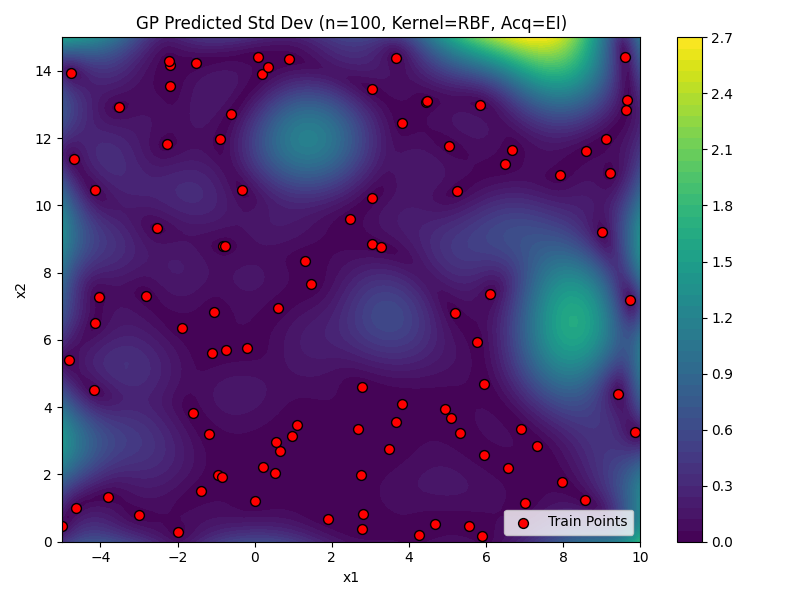
\includegraphics[width=\linewidth]{Task-02/images/gp_std_rbf_n100_EI.png}
    \caption{Std, $n=100$}
\end{subfigure}
\end{figure}

\subsection*{Kernel: Rational Quadratic}
\subsubsection*{Acquisition: Expected Improvement (EI)}
\begin{figure}[H]
\centering
\begin{subfigure}{0.3\textwidth}
  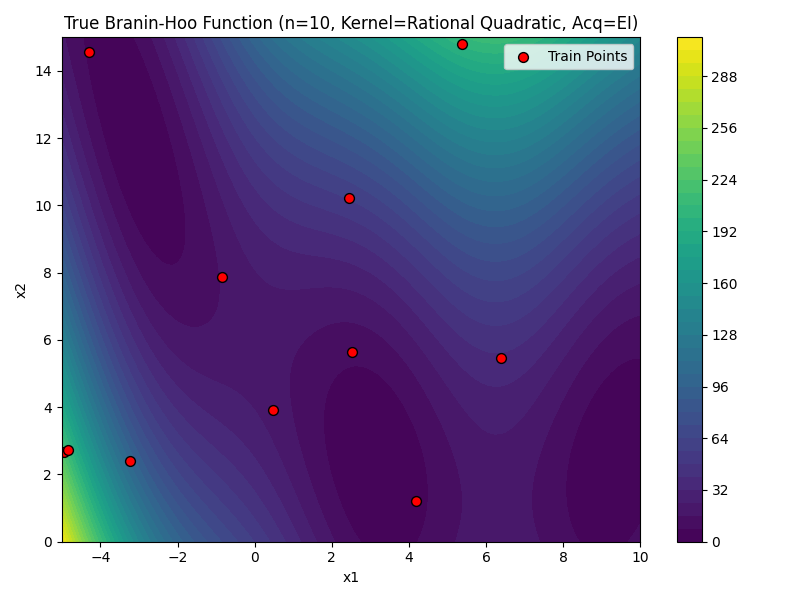
\includegraphics[width=\linewidth]{Task-02/images/true_function_rational_quadratic_n10_EI.png}
  \caption{True Branin-Hoo, $n=10$}
\end{subfigure}
\begin{subfigure}{0.3\textwidth}
    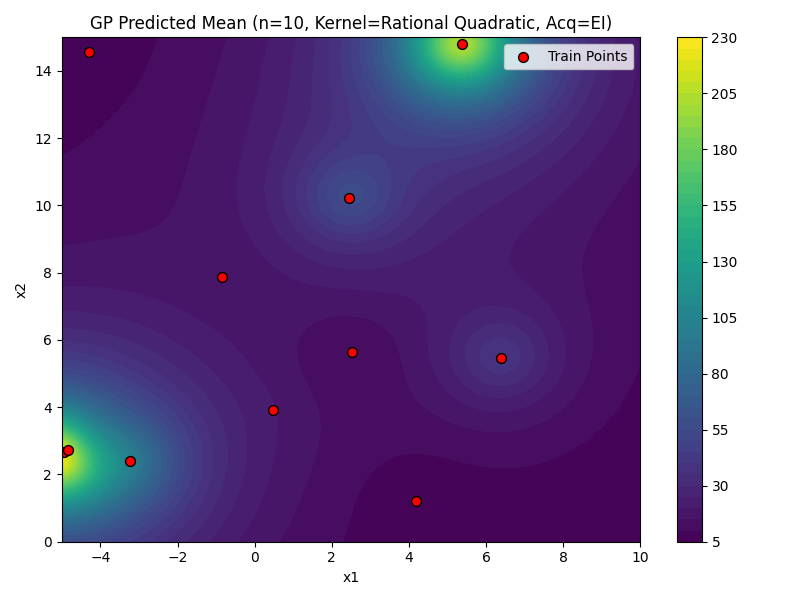
\includegraphics[width=\linewidth]{Task-02/images/gp_mean_rational_quadratic_n10_EI.png}
    \caption{Mean, $n=10$}
\end{subfigure}
\begin{subfigure}{0.3\textwidth}
    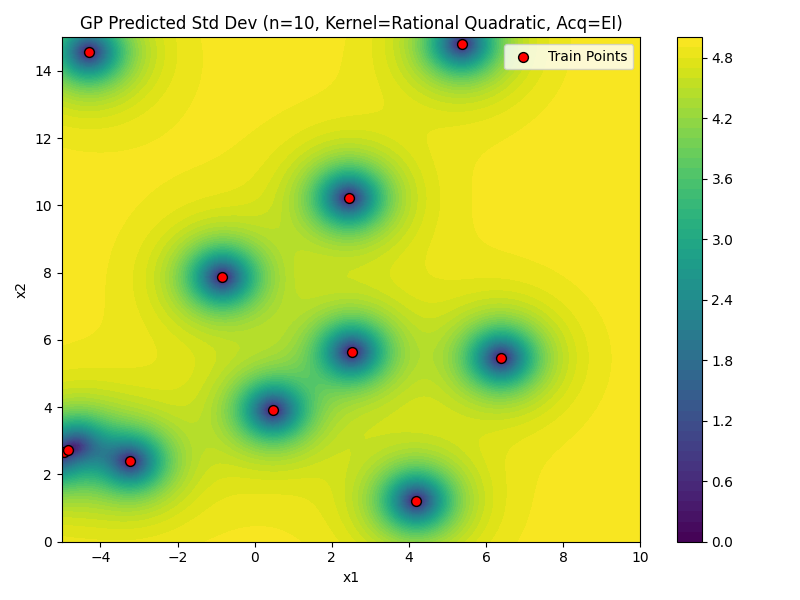
\includegraphics[width=\linewidth]{Task-02/images/gp_std_rational_quadratic_n10_EI.png}
    \caption{Std, $n=10$}
\end{subfigure}

\begin{subfigure}{0.3\textwidth}
  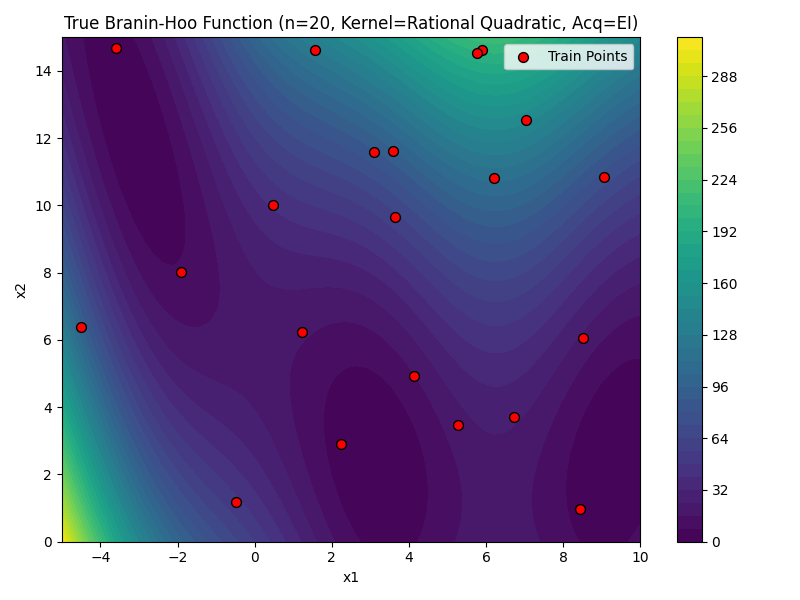
\includegraphics[width=\linewidth]{Task-02/images/true_function_rational_quadratic_n20_EI.png}
  \caption{True Branin-Hoo, $n=20$}
\end{subfigure}
\begin{subfigure}{0.3\textwidth}
    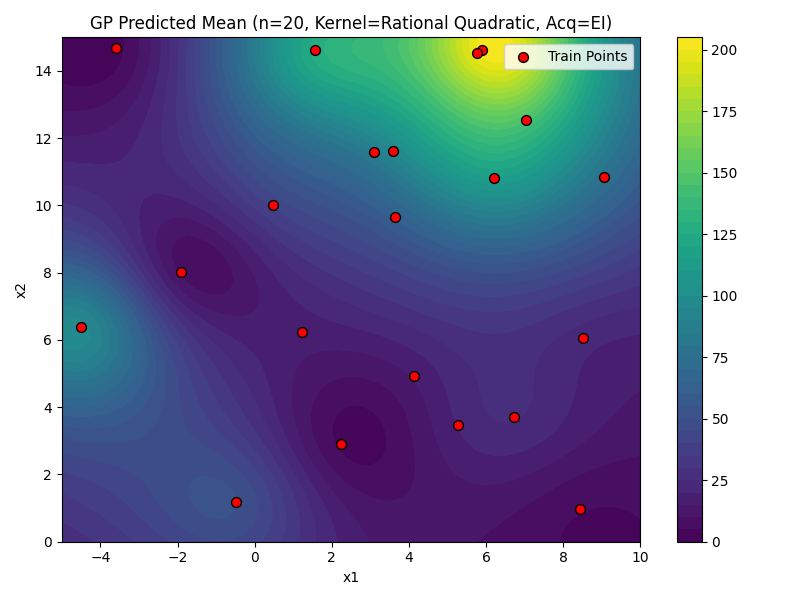
\includegraphics[width=\linewidth]{Task-02/images/gp_mean_rational_quadratic_n20_EI.png}
    \caption{Mean, $n=20$}
\end{subfigure}
\begin{subfigure}{0.3\textwidth}
    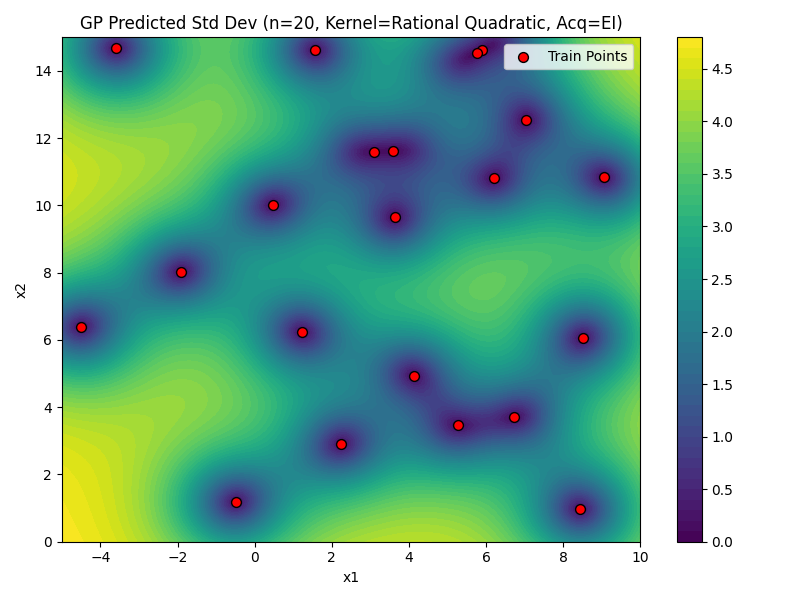
\includegraphics[width=\linewidth]{Task-02/images/gp_std_rational_quadratic_n20_EI.png}
    \caption{Std, $n=20$}
\end{subfigure}

\begin{subfigure}{0.3\textwidth}
  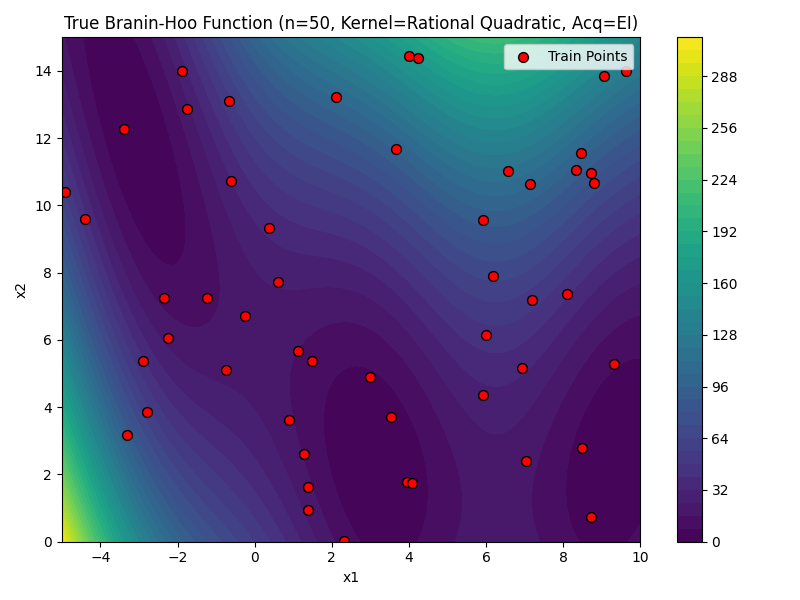
\includegraphics[width=\linewidth]{Task-02/images/true_function_rational_quadratic_n50_EI.png}
  \caption{True Branin-Hoo, $n=50$}
\end{subfigure}
\begin{subfigure}{0.3\textwidth}
    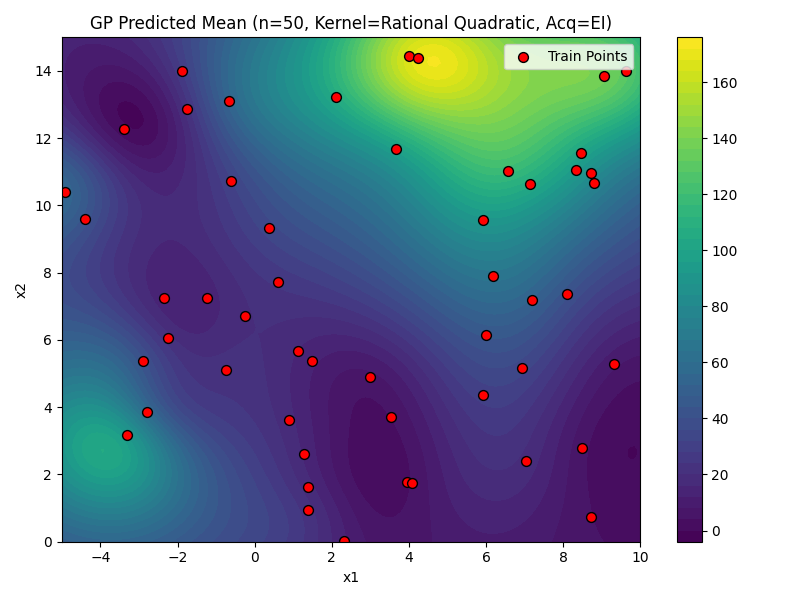
\includegraphics[width=\linewidth]{Task-02/images/gp_mean_rational_quadratic_n50_EI.png}
    \caption{Mean, $n=50$}
\end{subfigure}
\begin{subfigure}{0.3\textwidth}
    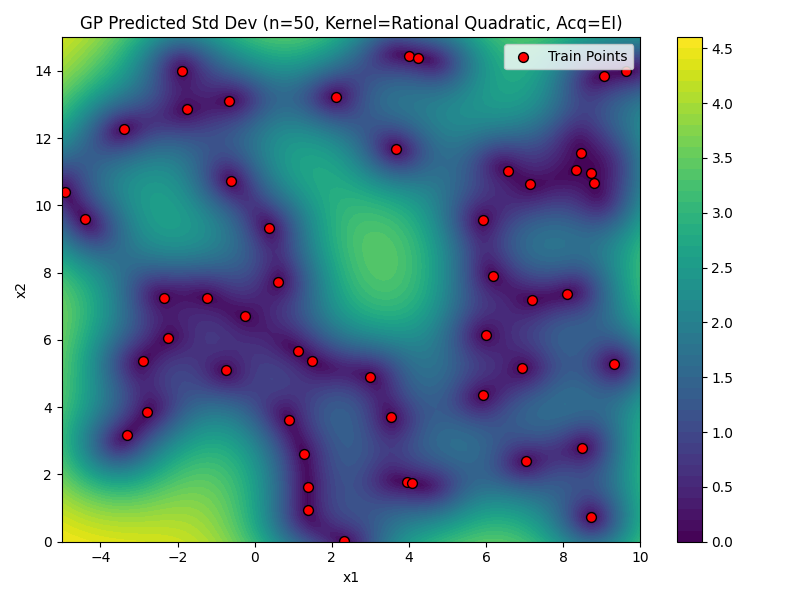
\includegraphics[width=\linewidth]{Task-02/images/gp_std_rational_quadratic_n50_EI.png}
    \caption{Std, $n=50$}
\end{subfigure}

\begin{subfigure}{0.3\textwidth}
  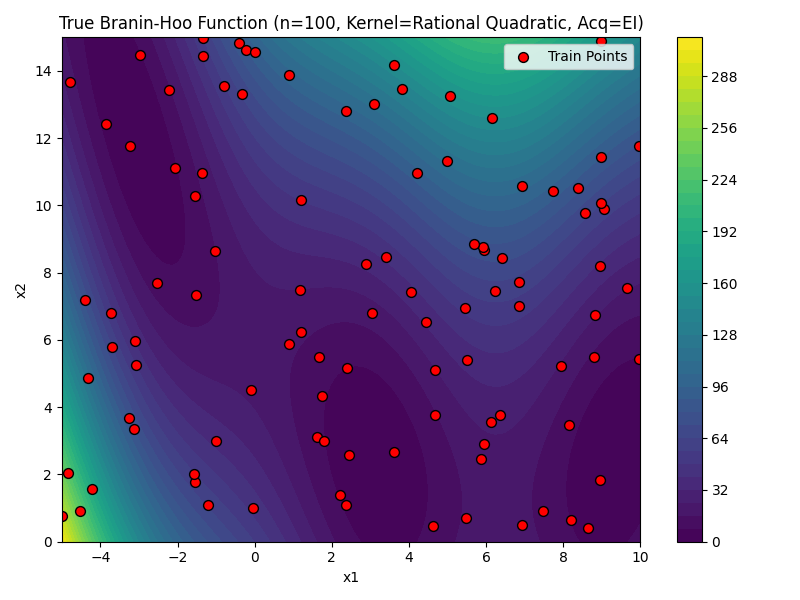
\includegraphics[width=\linewidth]{Task-02/images/true_function_rational_quadratic_n100_EI.png}
  \caption{True Branin-Hoo, $n=100$}
\end{subfigure}
\begin{subfigure}{0.3\textwidth}
    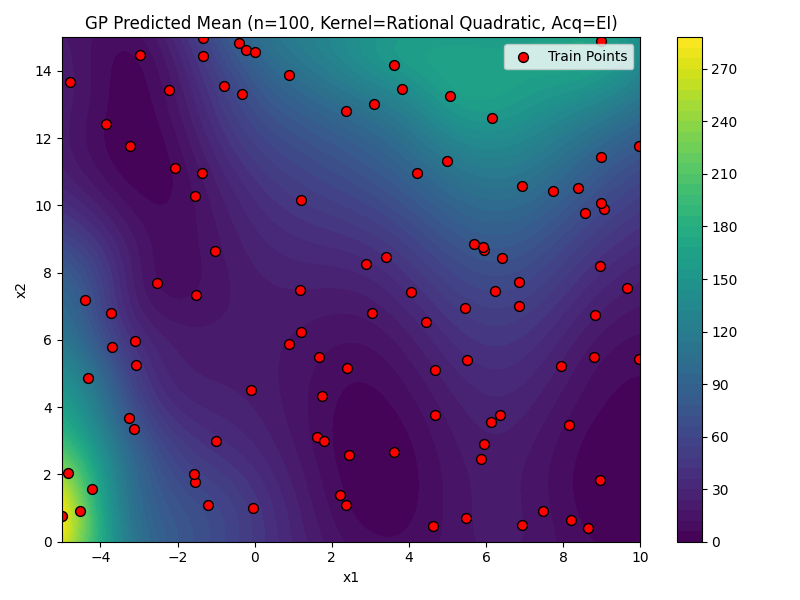
\includegraphics[width=\linewidth]{Task-02/images/gp_mean_rational_quadratic_n100_EI.png}
    \caption{Mean, $n=100$}
\end{subfigure}
\begin{subfigure}{0.3\textwidth}
    \includegraphics[width=\linewidth]{Task-02/images/gp_std_rational_quadratic_n100_EI.png}
    \caption{Std, $n=100$}
\end{subfigure}
\end{figure}

\subsection*{Kernel: Matérn}
\subsubsection*{Acquisition: Probability of Improvement (PI)}
\begin{figure}[H]
\centering

\begin{subfigure}{0.3\textwidth}
  \includegraphics[width=\linewidth]{Task-02/images/true_function_matern_n10_PI.png}
  \caption{True Branin-Hoo, $n=10$}
\end{subfigure}
\begin{subfigure}{0.3\textwidth}
    \includegraphics[width=\linewidth]{Task-02/images/gp_mean_matern_n10_PI.png}
    \caption{Mean, $n=10$}
\end{subfigure}
\begin{subfigure}{0.3\textwidth}
    \includegraphics[width=\linewidth]{Task-02/images/gp_std_matern_n10_PI.png}
    \caption{Std, $n=10$}
\end{subfigure}

\begin{subfigure}{0.3\textwidth}
  \includegraphics[width=\linewidth]{Task-02/images/true_function_matern_n20_PI.png}
  \caption{True Branin-Hoo, $n=20$}
\end{subfigure}
\begin{subfigure}{0.3\textwidth}
    \includegraphics[width=\linewidth]{Task-02/images/gp_mean_matern_n20_PI.png}
    \caption{Mean, $n=20$}
\end{subfigure}
\begin{subfigure}{0.3\textwidth}
    \includegraphics[width=\linewidth]{Task-02/images/gp_std_matern_n20_PI.png}
    \caption{Std, $n=20$}
\end{subfigure}

\begin{subfigure}{0.3\textwidth}
  \includegraphics[width=\linewidth]{Task-02/images/true_function_matern_n50_PI.png}
  \caption{True Branin-Hoo, $n=50$}
\end{subfigure}
\begin{subfigure}{0.3\textwidth}
    \includegraphics[width=\linewidth]{Task-02/images/gp_mean_matern_n50_PI.png}
    \caption{Mean, $n=50$}
\end{subfigure}
\begin{subfigure}{0.3\textwidth}
    \includegraphics[width=\linewidth]{Task-02/images/gp_std_matern_n50_PI.png}
    \caption{Std, $n=50$}
\end{subfigure}

\begin{subfigure}{0.3\textwidth}
  \includegraphics[width=\linewidth]{Task-02/images/true_function_matern_n100_PI.png}
  \caption{True Branin-Hoo, $n=100$}
\end{subfigure}
\begin{subfigure}{0.3\textwidth}
    \includegraphics[width=\linewidth]{Task-02/images/gp_mean_matern_n100_PI.png}
    \caption{Mean, $n=100$}
\end{subfigure}
\begin{subfigure}{0.3\textwidth}
    \includegraphics[width=\linewidth]{Task-02/images/gp_std_matern_n100_PI.png}
    \caption{Std, $n=100$}
\end{subfigure}
\end{figure}

\subsection*{Kernel: RBF}
\subsubsection*{Acquisition: Probability of Improvement (PI)}
\begin{figure}[H]
\centering

\begin{subfigure}{0.3\textwidth}
  \includegraphics[width=\linewidth]{Task-02/images/true_function_rbf_n10_PI.png}
  \caption{True Branin-Hoo, $n=10$}
\end{subfigure}
\begin{subfigure}{0.3\textwidth}
    \includegraphics[width=\linewidth]{Task-02/images/gp_mean_rbf_n10_PI.png}
    \caption{Mean, $n=10$}
\end{subfigure} 
\begin{subfigure}{0.3\textwidth}
    \includegraphics[width=\linewidth]{Task-02/images/gp_std_rbf_n10_PI.png}
    \caption{Std, $n=10$}
\end{subfigure}

\begin{subfigure}{0.3\textwidth}
  \includegraphics[width=\linewidth]{Task-02/images/true_function_rbf_n20_PI.png}
  \caption{True Branin-Hoo, $n=20$}
\end{subfigure}
\begin{subfigure}{0.3\textwidth}
    \includegraphics[width=\linewidth]{Task-02/images/gp_mean_rbf_n20_PI.png}
    \caption{Mean, $n=20$}
\end{subfigure}
\begin{subfigure}{0.3\textwidth}
    \includegraphics[width=\linewidth]{Task-02/images/gp_std_rbf_n20_PI.png}
    \caption{Std, $n=20$}
\end{subfigure}

\begin{subfigure}{0.3\textwidth}
  \includegraphics[width=\linewidth]{Task-02/images/true_function_rbf_n50_PI.png}
  \caption{True Branin-Hoo, $n=50$}
\end{subfigure}
\begin{subfigure}{0.3\textwidth}
    \includegraphics[width=\linewidth]{Task-02/images/gp_mean_rbf_n50_PI.png}
    \caption{Mean, $n=50$}
\end{subfigure}
\begin{subfigure}{0.3\textwidth}
    \includegraphics[width=\linewidth]{Task-02/images/gp_std_rbf_n50_PI.png}
    \caption{Std, $n=50$}
\end{subfigure}

\begin{subfigure}{0.3\textwidth}
  \includegraphics[width=\linewidth]{Task-02/images/true_function_rbf_n100_PI.png}
  \caption{True Branin-Hoo, $n=100$}
\end{subfigure}
\begin{subfigure}{0.3\textwidth}
    \includegraphics[width=\linewidth]{Task-02/images/gp_mean_rbf_n100_PI.png}
    \caption{Mean, $n=100$}
\end{subfigure}
\begin{subfigure}{0.3\textwidth}
    \includegraphics[width=\linewidth]{Task-02/images/gp_std_rbf_n100_PI.png}
    \caption{Std, $n=100$}
\end{subfigure}
\end{figure}

\subsection*{Kernel: Rational Quadratic}
\subsubsection*{Acquisition: Probability of Improvement (PI)}
\begin{figure}[H]
\centering

\begin{subfigure}{0.3\textwidth}
  \includegraphics[width=\linewidth]{Task-02/images/true_function_rational_quadratic_n10_PI.png}
  \caption{True Branin-Hoo, $n=10$}
\end{subfigure}
\begin{subfigure}{0.3\textwidth}
    \includegraphics[width=\linewidth]{Task-02/images/gp_mean_rational_quadratic_n10_PI.png}
    \caption{Mean, $n=10$}
\end{subfigure}
\begin{subfigure}{0.3\textwidth}
    \includegraphics[width=\linewidth]{Task-02/images/gp_std_rational_quadratic_n10_PI.png}
    \caption{Std, $n=10$}
\end{subfigure} 

\begin{subfigure}{0.3\textwidth}
  \includegraphics[width=\linewidth]{Task-02/images/true_function_rational_quadratic_n20_PI.png}
  \caption{True Branin-Hoo, $n=20$}
\end{subfigure}
\begin{subfigure}{0.3\textwidth}
    \includegraphics[width=\linewidth]{Task-02/images/gp_mean_rational_quadratic_n20_PI.png}
    \caption{Mean, $n=20$}
\end{subfigure}
\begin{subfigure}{0.3\textwidth}
    \includegraphics[width=\linewidth]{Task-02/images/gp_std_rational_quadratic_n20_PI.png}
    \caption{Std, $n=20$}
\end{subfigure}

\begin{subfigure}{0.3\textwidth}
  \includegraphics[width=\linewidth]{Task-02/images/true_function_rational_quadratic_n50_PI.png}
  \caption{True Branin-Hoo, $n=50$}
\end{subfigure}
\begin{subfigure}{0.3\textwidth}
    \includegraphics[width=\linewidth]{Task-02/images/gp_mean_rational_quadratic_n50_PI.png}
    \caption{Mean, $n=50$}
\end{subfigure}
\begin{subfigure}{0.3\textwidth}
    \includegraphics[width=\linewidth]{Task-02/images/gp_std_rational_quadratic_n50_PI.png}
    \caption{Std, $n=50$}
\end{subfigure}

\begin{subfigure}{0.3\textwidth}
  \includegraphics[width=\linewidth]{Task-02/images/true_function_rational_quadratic_n100_PI.png}
  \caption{True Branin-Hoo, $n=100$}
\end{subfigure}
\begin{subfigure}{0.3\textwidth}
    \includegraphics[width=\linewidth]{Task-02/images/gp_mean_rational_quadratic_n100_PI.png}
    \caption{Mean, $n=100$}
\end{subfigure}
\begin{subfigure}{0.3\textwidth}
    \includegraphics[width=\linewidth]{Task-02/images/gp_std_rational_quadratic_n100_PI.png}
    \caption{Std, $n=100$}
\end{subfigure}
\end{figure}

\subsection*{Kernel: Matérn}
\subsubsection*{Acquisition: Random}
\begin{figure}[H]
\centering  

\begin{subfigure}{0.3\textwidth}
  \includegraphics[width=\linewidth]{Task-02/images/true_function_matern_n10_random.png}
  \caption{True Branin-Hoo, $n=10$}
\end{subfigure}
\begin{subfigure}{0.3\textwidth}
    \includegraphics[width=\linewidth]{Task-02/images/gp_mean_matern_n10_random.png}
    \caption{Mean, $n=10$}
\end{subfigure}
\begin{subfigure}{0.3\textwidth}
    \includegraphics[width=\linewidth]{Task-02/images/gp_std_matern_n10_random.png}
    \caption{Std, $n=10$}
\end{subfigure}

\begin{subfigure}{0.3\textwidth}
  \includegraphics[width=\linewidth]{Task-02/images/true_function_matern_n20_random.png}
  \caption{True Branin-Hoo, $n=20$}
\end{subfigure}
\begin{subfigure}{0.3\textwidth}
    \includegraphics[width=\linewidth]{Task-02/images/gp_mean_matern_n20_random.png}
    \caption{Mean, $n=20$}
\end{subfigure}
\begin{subfigure}{0.3\textwidth}
    \includegraphics[width=\linewidth]{Task-02/images/gp_std_matern_n20_random.png}
    \caption{Std, $n=20$}
\end{subfigure}

\begin{subfigure}{0.3\textwidth}
  \includegraphics[width=\linewidth]{Task-02/images/true_function_matern_n50_random.png}
  \caption{True Branin-Hoo, $n=50$}
\end{subfigure}
\begin{subfigure}{0.3\textwidth}
    \includegraphics[width=\linewidth]{Task-02/images/gp_mean_matern_n50_random.png}
    \caption{Mean, $n=50$}
\end{subfigure} 
\begin{subfigure}{0.3\textwidth}
    \includegraphics[width=\linewidth]{Task-02/images/gp_std_matern_n50_random.png}
    \caption{Std, $n=50$}
\end{subfigure}

\begin{subfigure}{0.3\textwidth}
  \includegraphics[width=\linewidth]{Task-02/images/true_function_matern_n100_random.png}
  \caption{True Branin-Hoo, $n=100$}
\end{subfigure}
\begin{subfigure}{0.3\textwidth}
    \includegraphics[width=\linewidth]{Task-02/images/gp_mean_matern_n100_random.png}
    \caption{Mean, $n=100$}
\end{subfigure}
\begin{subfigure}{0.3\textwidth}
    \includegraphics[width=\linewidth]{Task-02/images/gp_std_matern_n100_random.png}
    \caption{Std, $n=100$}
\end{subfigure}
\end{figure}

\subsection*{Kernel: RBF}
\subsubsection*{Acquisition: Random}
\begin{figure}[H]
\centering

\begin{subfigure}{0.3\textwidth}
  \includegraphics[width=\linewidth]{Task-02/images/true_function_rbf_n10_random.png}
  \caption{True Branin-Hoo, $n=10$}
\end{subfigure}
\begin{subfigure}{0.3\textwidth}
    \includegraphics[width=\linewidth]{Task-02/images/gp_mean_rbf_n10_random.png}
    \caption{Mean, $n=10$}
\end{subfigure}
\begin{subfigure}{0.3\textwidth}
    \includegraphics[width=\linewidth]{Task-02/images/gp_std_rbf_n10_random.png}
    \caption{Std, $n=10$}
\end{subfigure}

\begin{subfigure}{0.3\textwidth}
  \includegraphics[width=\linewidth]{Task-02/images/true_function_rbf_n20_random.png}
  \caption{True Branin-Hoo, $n=20$}
\end{subfigure}
\begin{subfigure}{0.3\textwidth}
    \includegraphics[width=\linewidth]{Task-02/images/gp_mean_rbf_n20_random.png}
    \caption{Mean, $n=20$}
\end{subfigure}
\begin{subfigure}{0.3\textwidth}
    \includegraphics[width=\linewidth]{Task-02/images/gp_std_rbf_n20_random.png}
    \caption{Std, $n=20$}
\end{subfigure}

\begin{subfigure}{0.3\textwidth}
  \includegraphics[width=\linewidth]{Task-02/images/true_function_rbf_n50_random.png}
  \caption{True Branin-Hoo, $n=50$}
\end{subfigure}
\begin{subfigure}{0.3\textwidth}
    \includegraphics[width=\linewidth]{Task-02/images/gp_mean_rbf_n50_random.png}
    \caption{Mean, $n=50$}
\end{subfigure}
\begin{subfigure}{0.3\textwidth}
    \includegraphics[width=\linewidth]{Task-02/images/gp_std_rbf_n50_random.png}
    \caption{Std, $n=50$}
\end{subfigure}

\begin{subfigure}{0.3\textwidth}
  \includegraphics[width=\linewidth]{Task-02/images/true_function_rbf_n100_random.png}
  \caption{True Branin-Hoo, $n=100$}
\end{subfigure}
\begin{subfigure}{0.3\textwidth}
    \includegraphics[width=\linewidth]{Task-02/images/gp_mean_rbf_n100_random.png}
    \caption{Mean, $n=100$}
\end{subfigure}
\begin{subfigure}{0.3\textwidth}
    \includegraphics[width=\linewidth]{Task-02/images/gp_std_rbf_n100_random.png}
    \caption{Std, $n=100$}  
\end{subfigure}
\end{figure}

\subsection*{Kernel: Rational Quadratic}
\subsubsection*{Acquisition: Random}
\begin{figure}[H]
\centering
\begin{subfigure}{0.3\textwidth}
  \includegraphics[width=\linewidth]{Task-02/images/true_function_rational_quadratic_n10_random.png}
  \caption{True Branin-Hoo, $n=10$}
\end{subfigure}
\begin{subfigure}{0.3\textwidth}
    \includegraphics[width=\linewidth]{Task-02/images/gp_mean_rational_quadratic_n10_random.png}
    \caption{Mean, $n=10$}
\end{subfigure}
\begin{subfigure}{0.3\textwidth}
    \includegraphics[width=\linewidth]{Task-02/images/gp_std_rational_quadratic_n10_random.png}
    \caption{Std, $n=10$}
\end{subfigure}

\begin{subfigure}{0.3\textwidth}
  \includegraphics[width=\linewidth]{Task-02/images/true_function_rational_quadratic_n20_random.png}
  \caption{True Branin-Hoo, $n=20$}
\end{subfigure}
\begin{subfigure}{0.3\textwidth}
    \includegraphics[width=\linewidth]{Task-02/images/gp_mean_rational_quadratic_n20_random.png}
    \caption{Mean, $n=20$}
\end{subfigure}
\begin{subfigure}{0.3\textwidth}
    \includegraphics[width=\linewidth]{Task-02/images/gp_std_rational_quadratic_n20_random.png}
    \caption{Std, $n=20$}
\end{subfigure}

\begin{subfigure}{0.3\textwidth}
  \includegraphics[width=\linewidth]{Task-02/images/true_function_rational_quadratic_n50_random.png}
  \caption{True Branin-Hoo, $n=50$}
\end{subfigure}
\begin{subfigure}{0.3\textwidth}
    \includegraphics[width=\linewidth]{Task-02/images/gp_mean_rational_quadratic_n50_random.png}
    \caption{Mean, $n=50$}
\end{subfigure}
\begin{subfigure}{0.3\textwidth}
    \includegraphics[width=\linewidth]{Task-02/images/gp_std_rational_quadratic_n50_random.png}
    \caption{Std, $n=50$}
\end{subfigure}

\begin{subfigure}{0.3\textwidth}
  \includegraphics[width=\linewidth]{Task-02/images/true_function_rational_quadratic_n100_random.png}
  \caption{True Branin-Hoo, $n=100$}
\end{subfigure}
\begin{subfigure}{0.3\textwidth}
    \includegraphics[width=\linewidth]{Task-02/images/gp_mean_rational_quadratic_n100_random.png}
    \caption{Mean, $n=100$}
\end{subfigure}
\begin{subfigure}{0.3\textwidth}
    \includegraphics[width=\linewidth]{Task-02/images/gp_std_rational_quadratic_n100_random.png}
    \caption{Std, $n=100$}
\end{subfigure} 
\end{figure}

\subsection*{Analysis of Model Performance}

We analyze the Gaussian Process (GP) model performance in approximating the Branin-Hoo function. The evaluation is based on a comparison across different kernels (RBF, Matérn, Rational Quadratic), training sample sizes ($n = 10, 20, 50, 100$), and acquisition strategies (Random, Expected Improvement (EI), Probability of Improvement (PI)).

\textbf{1. Effect of Sample Size ($n$):}
\begin{itemize}
    \item For all kernel-acquisition combinations, increasing $n$ leads to visibly better approximations of the Branin-Hoo function.
    \item At $n = 10$, the predicted mean is not very naccurate, with significant deviations from the true function and high uncertainty in most regions.
    \item At $n = 20$, the predicted mean is improves in accuracy, with minor deviations from the true function but still having uncertainty in some regions.
    \item At $n = 50$, the predicted mean starts resembling the true function across kernels, with a noticeable reduction in standard deviation.
    \item At $n = 100$, predictions closely match the Branin-Hoo landscape, and uncertainty is minimized in most areas.
\end{itemize}

\textbf{2. Kernel Performance:}
\begin{itemize}
    \item \textbf{Matérn Kernel:} Performs best overall. Even at $n = 20$, the predicted mean aligns reasonably with the true function, and uncertainty is focused only in unexplored regions. Especially when combined with EI or PI, this kernel consistently balances smoothness and flexibility.
    \item \textbf{RBF Kernel:} Gives smooth approximations, but might over-smoothen regions with sharp curvature. The uncertainty bands are tight even when the prediction is visibly incorrect, especially at low $n$, indicating overconfidence.
    \item \textbf{Rational Quadratic Kernel:} Shows higher uncertainty in flatter regions compared to RBF, but slightly better adaptability to varying smoothness. At $n = 50$ and $n = 100$, performance becomes comparable to Matérn.
\end{itemize}

\textbf{3. Acquisition Function Comparison:}
\begin{itemize}
    \item \textbf{Expected Improvement (EI):} Consistently provides the best approximations across all sample sizes and kernels. Even at $n = 20$, models with EI have good coverage of the global minima and reduced uncertainty in key regions.
    \item \textbf{Probability of Improvement (PI):} Performs well but slightly worse than EI. It tends to exploit known regions and sometimes misses exploring uncertain areas, visible in the standard deviation plots.
    \item \textbf{Random Acquisition:} Performs the worst at small $n$. The predicted mean often misses important features of the true function, and uncertainty remains high across the domain. Only at $n = 100$ does performance begin to resemble structured acquisition strategies.
\end{itemize}

\subsection*{Conclusion}

From the plot-based results, we conclude that:
\begin{itemize}
    \item The \textbf{Matérn kernel}, when combined with \textbf{Expected Improvement}, consistently yields the most accurate and uncertainty-aware approximation of the Branin-Hoo function.
    \item Increasing the number of training samples improves approximation quality and reduces uncertainty.
    \item Acquisition strategy has a substantial impact—\textbf{Random acquisition} fails to explore key regions efficiently, whereas \textbf{EI} strategically balances exploration and exploitation.
\end{itemize}


\end{document}